\chapter{Cherenkov angle resolution by mirror-pair}
In this chapter the Cherenkov angle resolution per mirror-pair is studied.\\
The 2D histograms of the Cherenkov angle resolution $\Delta \theta$ vs. azimuthal angle $\Phi$ for fully aligned mirrors are projected onto the Cherenkov angle resolution. Then a function consisting of a Gaussian representing the signal contribution and a polynomial of order 2 representing the background contribution is fitted to the Cherenkov angle resolution distribution: 
\begin{equation}
f(x) = a \cdot e^{-0.5 \cdot \left( \frac{x - \mu}{\sigma}\right)^2} + b + c \cdot x + d \cdot x^2
\label{eq:1}
\end{equation}
($a$, $b$, $c$, $d$, $\mu$ and $\sigma$ are determined by the fit).\\
The width of the fitted Gaussian represents the Cherenkov angle resolution.\\
\begin{figure}[!h]
	\vspace*{-0.cm}
	\begin{center}
		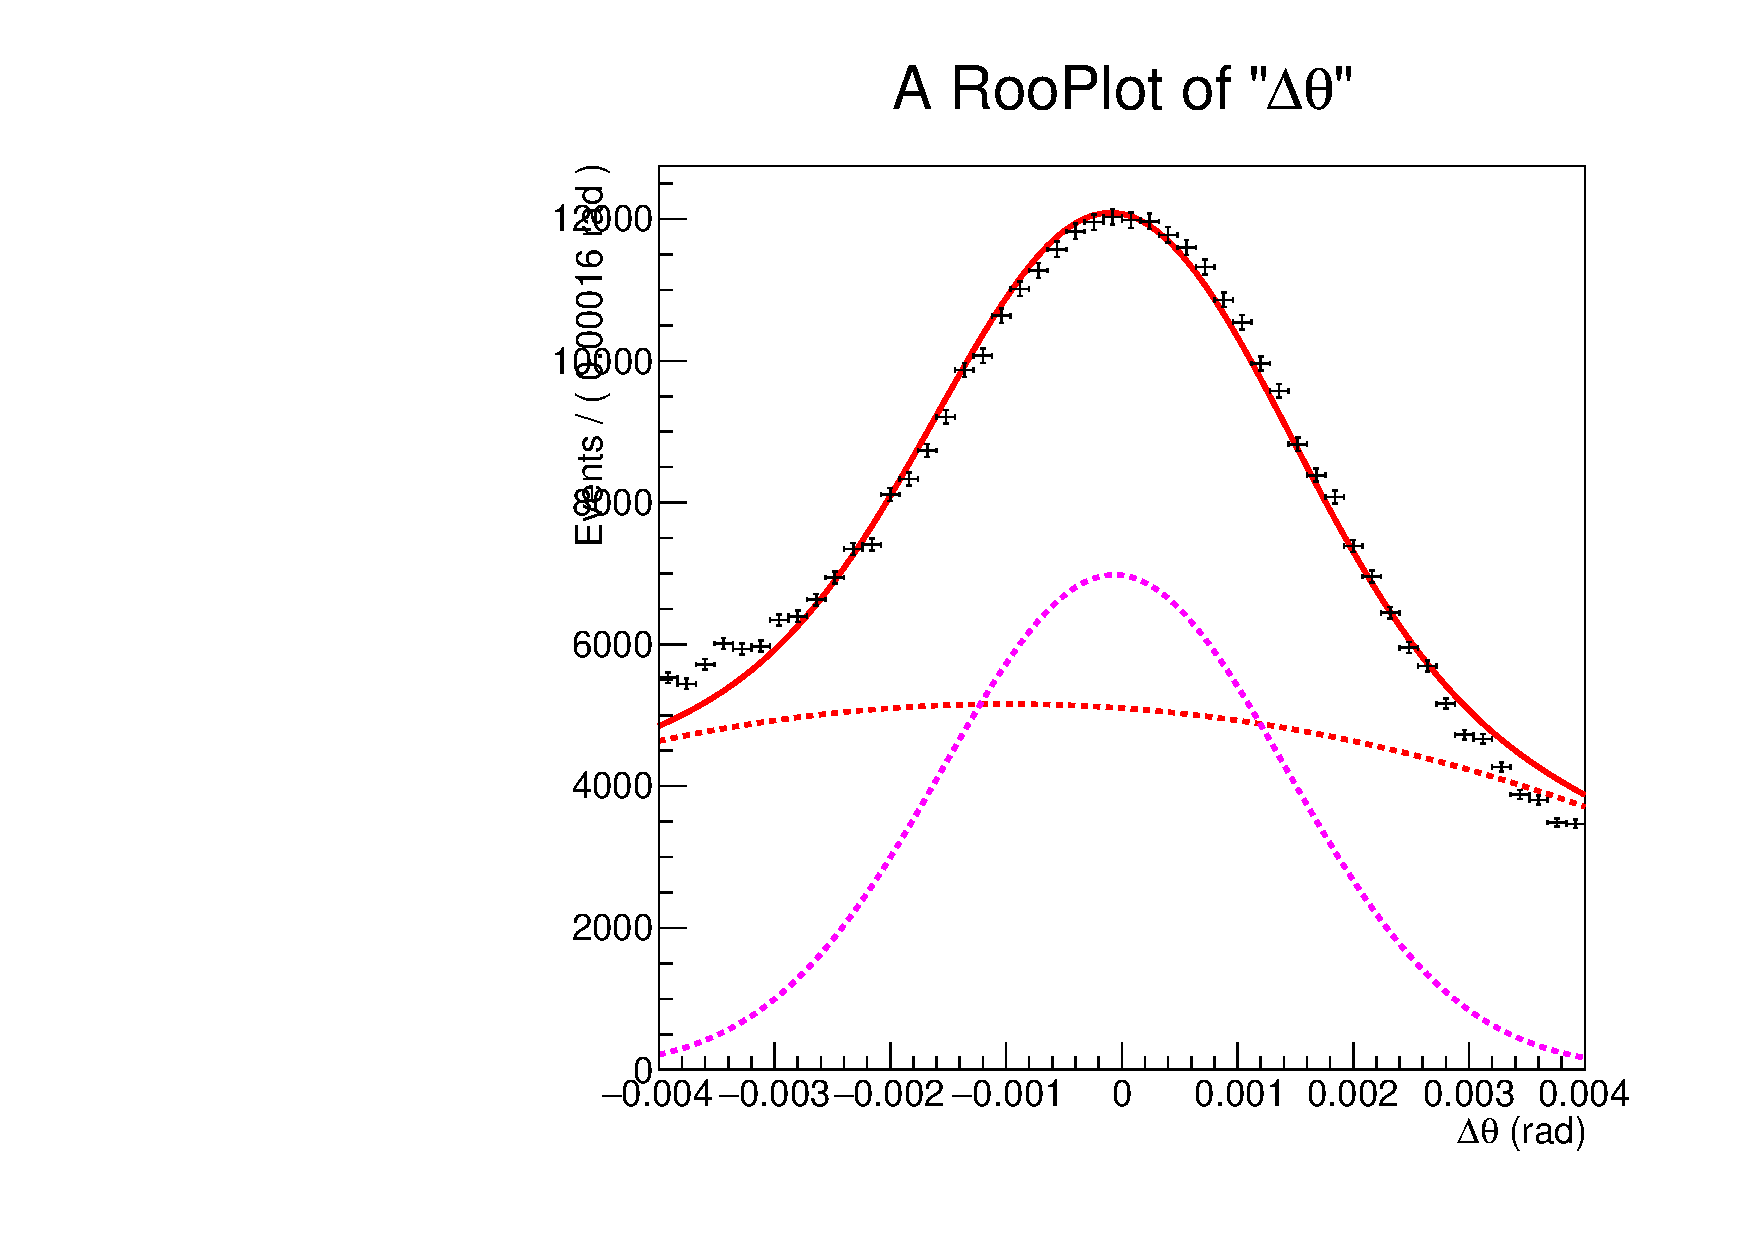
\includegraphics[width=0.7\textwidth]{rootest.pdf}
		\vspace*{-1.cm}
	\end{center}
	\caption{\textit{Example of a fit to the Cherenkov angle resolution distribution for RICH1. Dotted purple line: signal Gaussian, dotted red line: polynomial order 2 background,  solid red line: total function, black points: data points.} }
	\label{fig:fitfunc}
\end{figure}

\section{RICH1}

\subsection{Introduction}
Each secondary mirror of RICH1 only receives photons from one primary mirror. Therefore the primary mirror positions are fixed during the alignment procedure and any possible misalignments will be compensated by tilts in the secondary mirrors. Figure \ref{fig:rich1mirr} shows the primary and secondary mirrors of RICH1. \\
\begin{figure}[!h]
	\vspace*{-0.cm}
	\begin{center}
		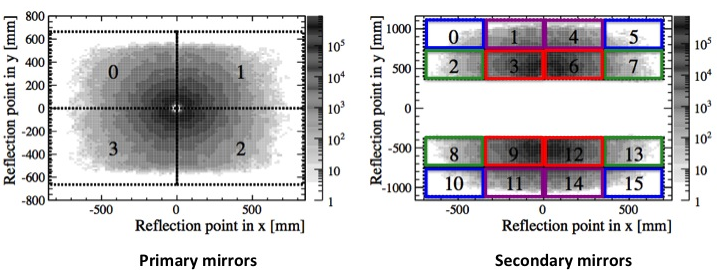
\includegraphics[width=1.\textwidth]{rich1mirrors.png}
		\vspace*{-1.5cm}
	\end{center}
	\caption{\textit{Primary and secondary mirrors of RICH1. Blue: secondary mirrors in category 1 (outer corners), red: secondary mirrors in category 2 (inner corners), purple: secondary mirrors in category 3 (middle in top + bottom row), green secondary mirrors in category 4 (middle in left + right column).}}
	\label{fig:rich1mirr}
\end{figure}
Mirror-pairs are denoted by a four-digit number where the first two numbers refer to the primary mirror and the last two to the secondary mirror, e.g. 0001 refers to the pair formed by the top left primary mirror (number 00) and the second secondary mirror in the top row (number 01).\\
\\
In the following different quantities are compared by mirror-pair. In order to make the information as accessible as possible the values will be shown in heatmaps where each bin will represent a mirror pair. For RICH1 the bins are basically just the schematic position of the secondary mirrors as shown in Figure \ref{fig:rich1mirr}.\\


\subsection{Cherenkov angle resolution by mirror-pair}
Here the Cherenkov angle resolution for each mirror-pair is shown for three different alignments which actually converged. \\
The \textbf{first alignment} is the very first alignment made on 2015 data that converged. It was made online on the 11.07.2015 on early measurement data (mag down). It started from an attempted alignment on 2015 data with MDCS correction that never converged. This alignment converged after 4 iterations and is currently used in the database.\\
The \textbf{second alignment} was made on three fills of mag up data on the 09.09.2015. The alignment procedure started with the first alignment and converged after 2 iterations.\\
The \textbf{third alignment} was made on the three fills of mag up data that followed those for the second alignment. It was made starting from the second alignment and converged after 2 iterations.\\
Figure \ref{fig:rich1maps} shows the Cherenkov angle resolution at the end of each alignment for each mirror pair in $mrad$. The value in the title of each plot is the absolute Cherenkov angle resolution.\\
\begin{figure}[!h]
	\vspace*{-0.cm}
	\begin{center}
		\subfigure{ 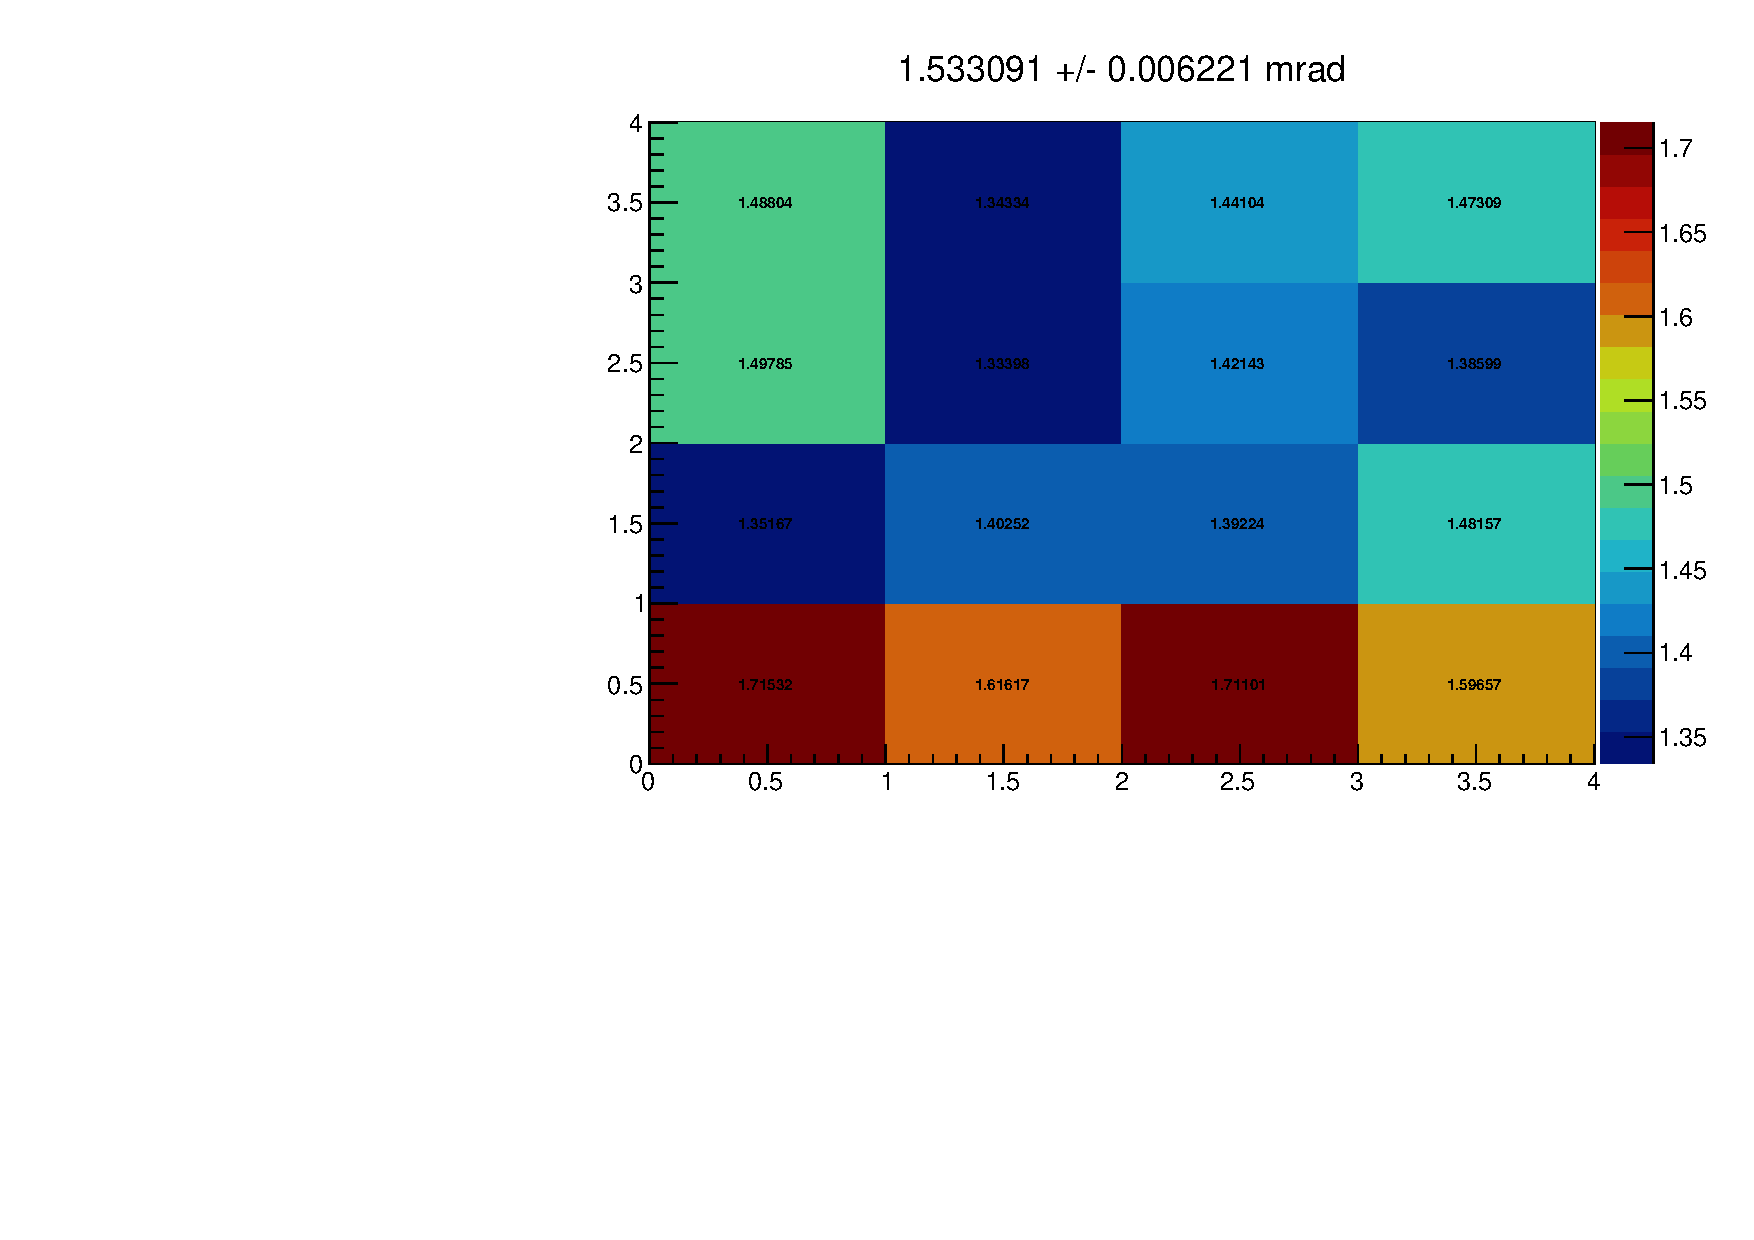
\includegraphics[width=0.48 \textwidth] {map_rich1_11072015.pdf}}
		\subfigure{ 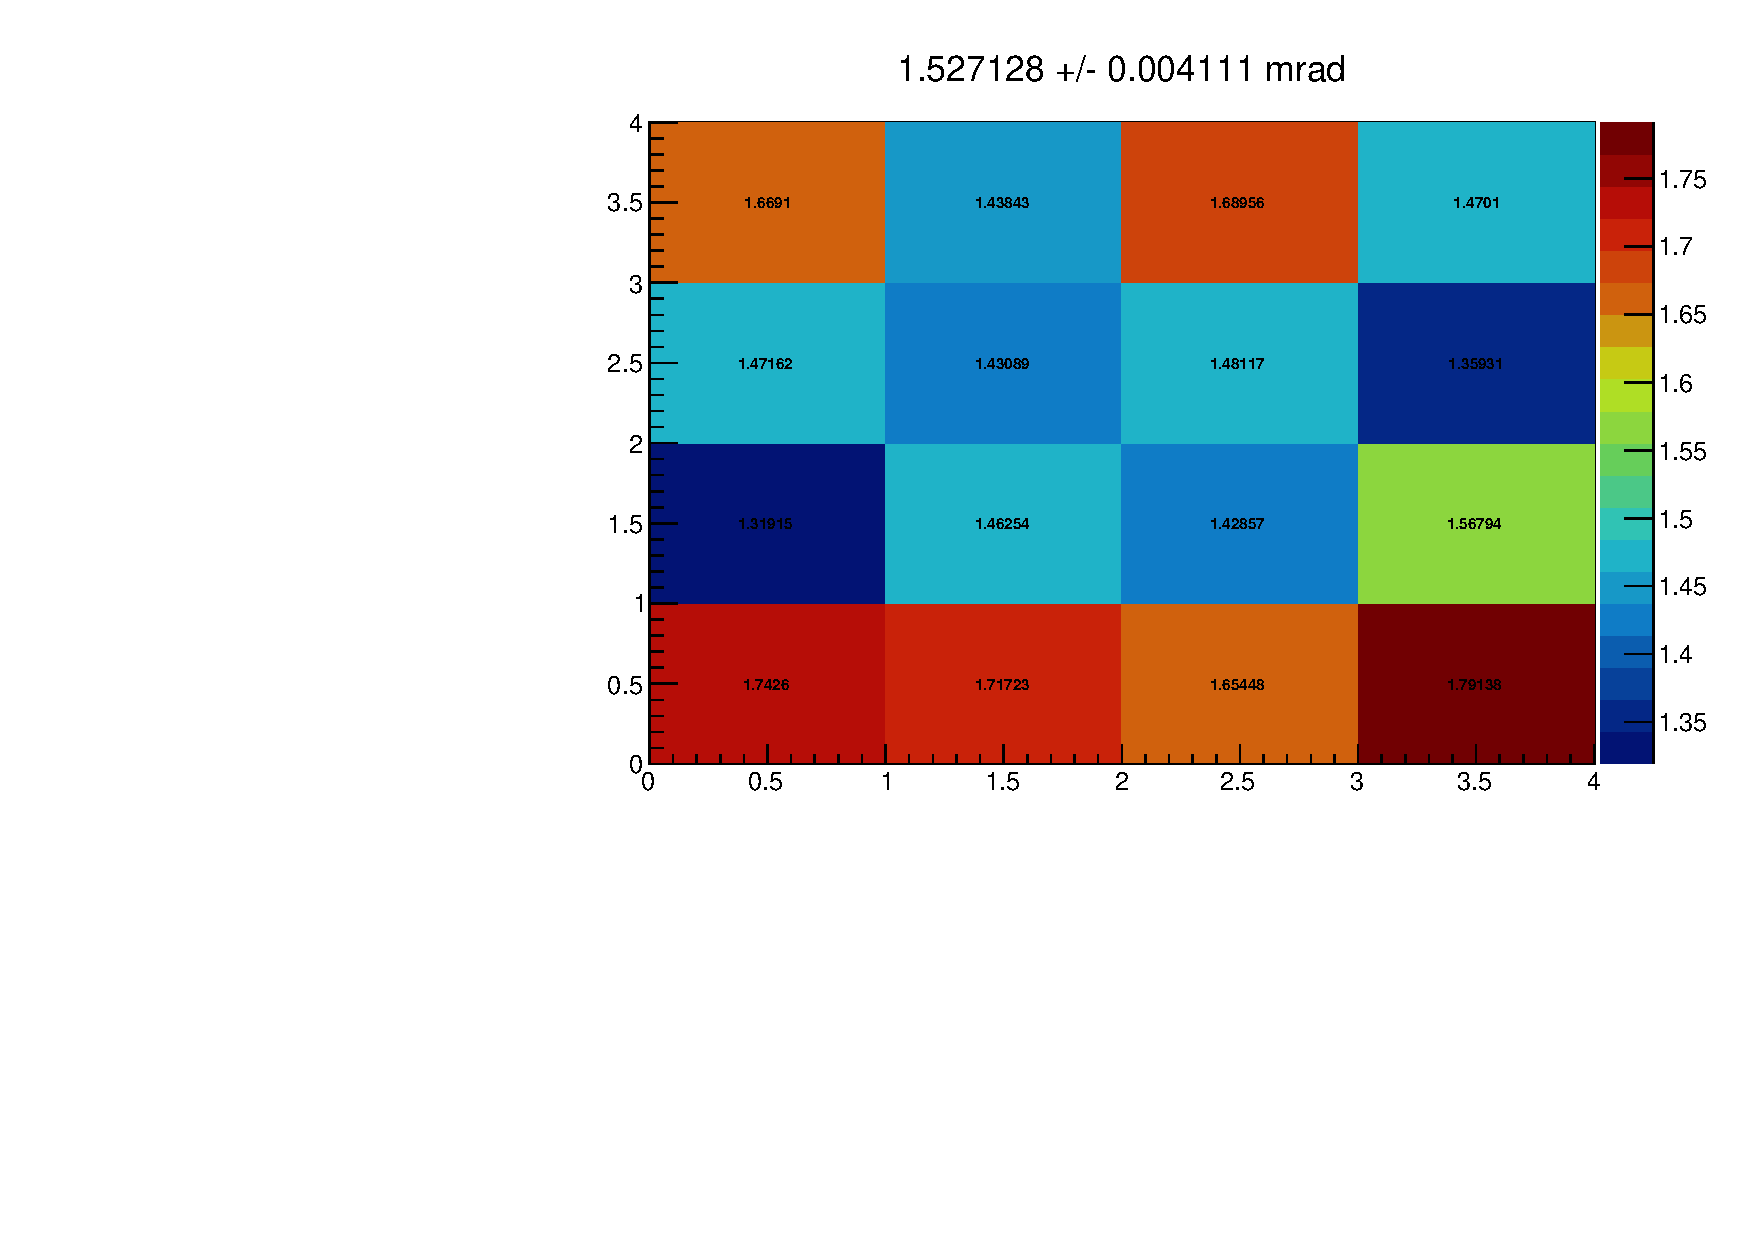
\includegraphics[width=0.48 \textwidth] {map_rich1_09092015.pdf}}
		\subfigure{ 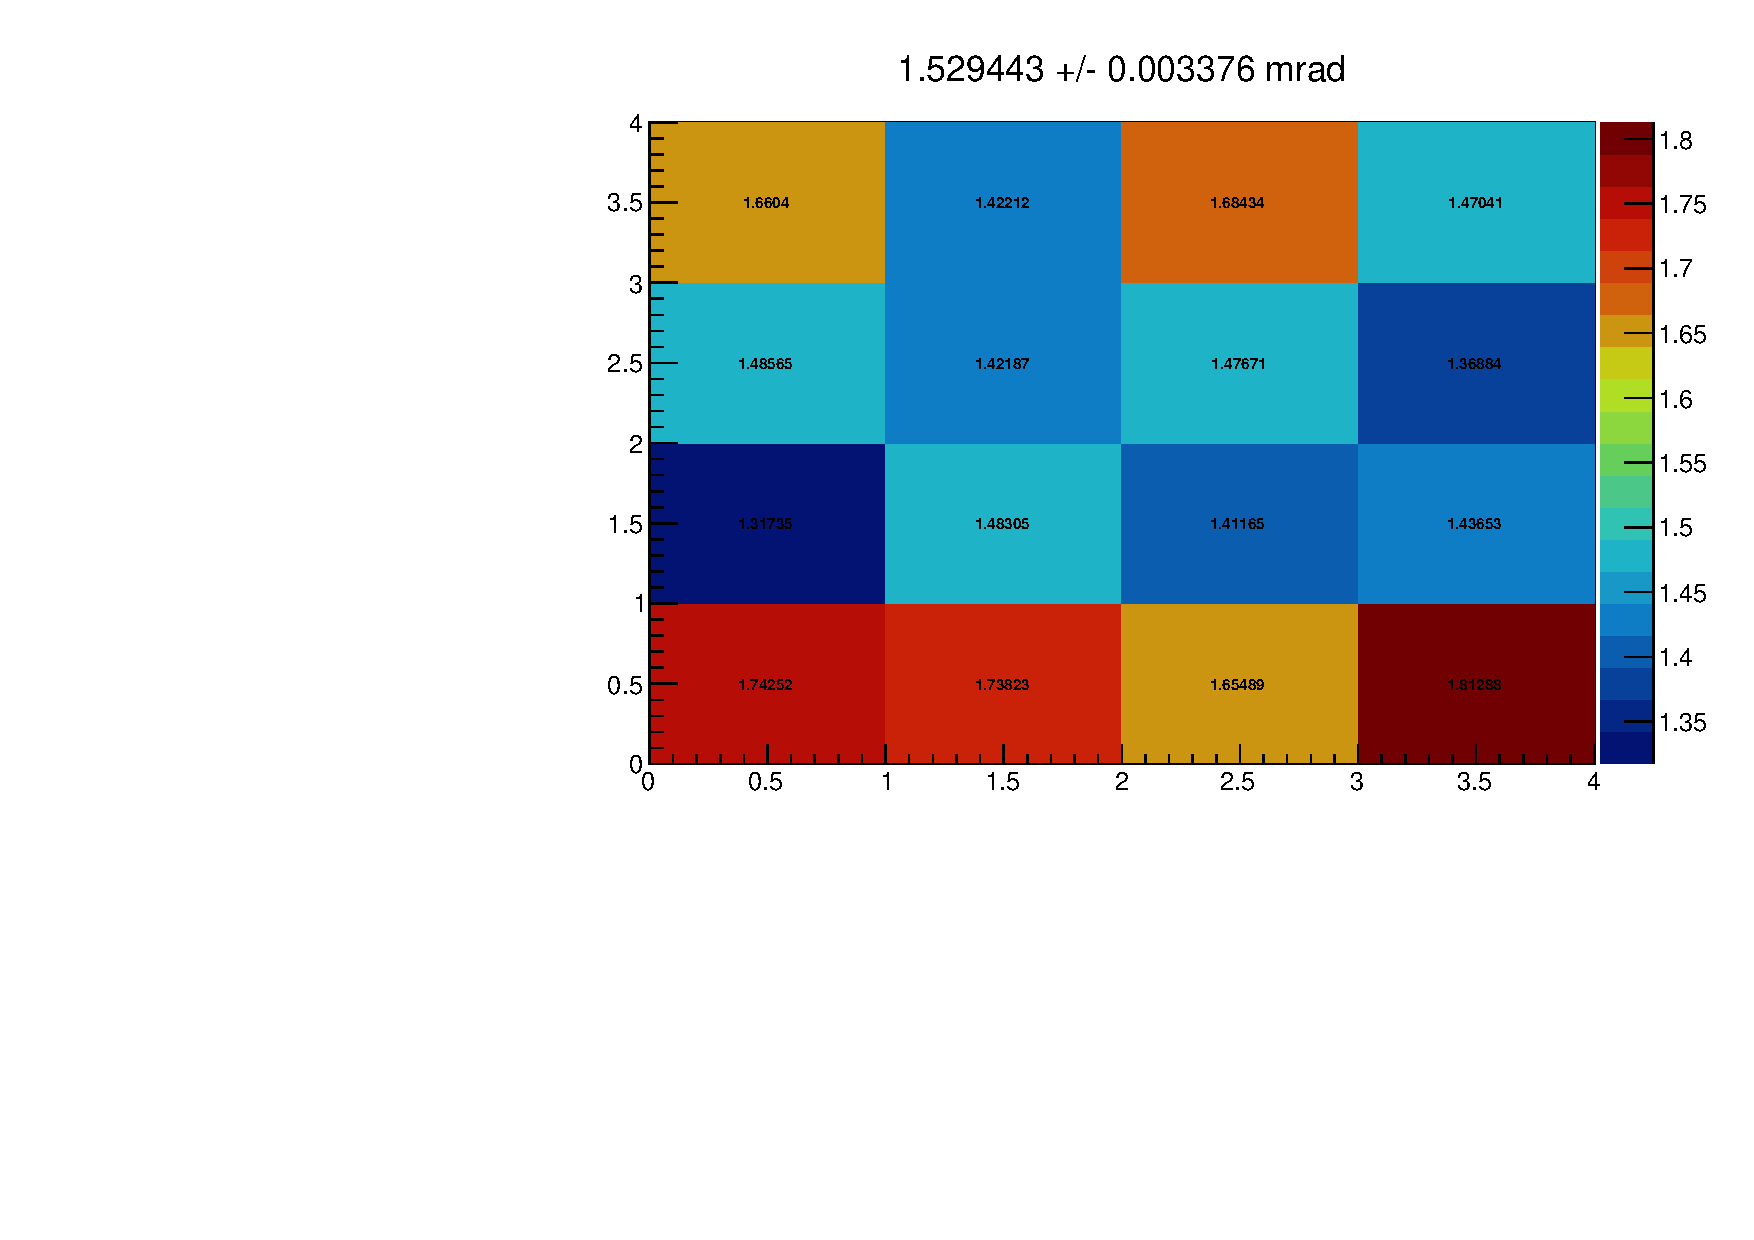
\includegraphics[width=0.48 \textwidth] {map_rich1_10092015.pdf}}
		\vspace*{-0.5cm}
	\end{center}
	\caption{\textit{Cherenkov angle resolution for each mirror-pair in RICH1 in mrad. Top left:} \textbf{first alignment}\textit{; top right:} \textbf{second alignment}\textit{; bottom:} \textbf{third alignment}\textit{. The value in the title of each plot is the absolute Cherenkov angle resolution. } }
	\label{fig:rich1maps}
\end{figure}


Note that the second and third alignments are very similar. They were performed on consecutive fills and in the third alignment only one mirror changed and that only the minimal tilt of $0.1\, mrad$.\\


\subsection{Change of Cherenkov angle resolution over alignment}
Here the change of the Cherenkov angle resolution between the first and the last iteration of the above three alignments is shown.\\
Figure \ref{fig:rich1del} shows the change in Cherenkov angle resolution for each mirror pair in $mrad$. The value in the title of each plot is the absolute change in Cherenkov angle resolution.\\
\begin{figure}[!h]
	\vspace*{-0.cm}
	\begin{center}
		\subfigure{ 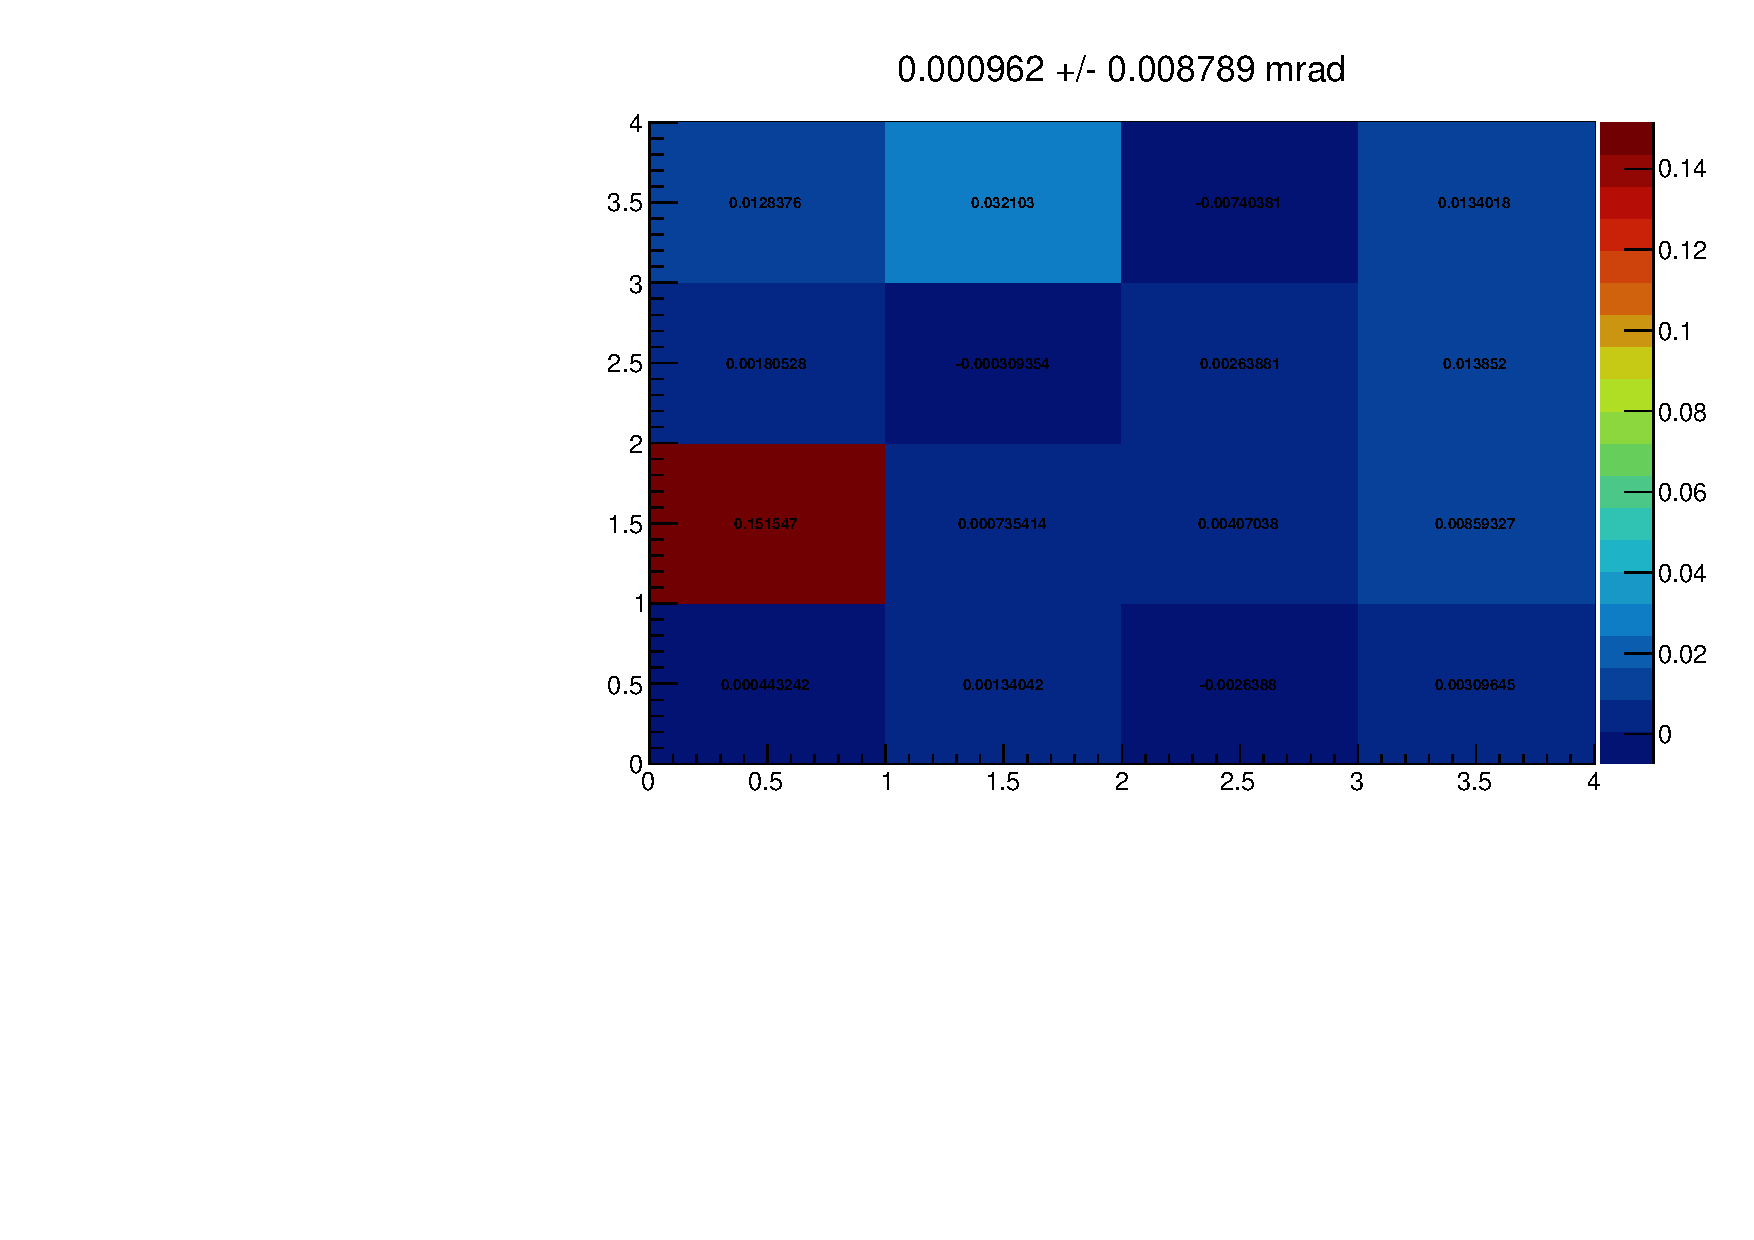
\includegraphics[width=0.48 \textwidth] {del_rich1_11072015.pdf}}
		\subfigure{ 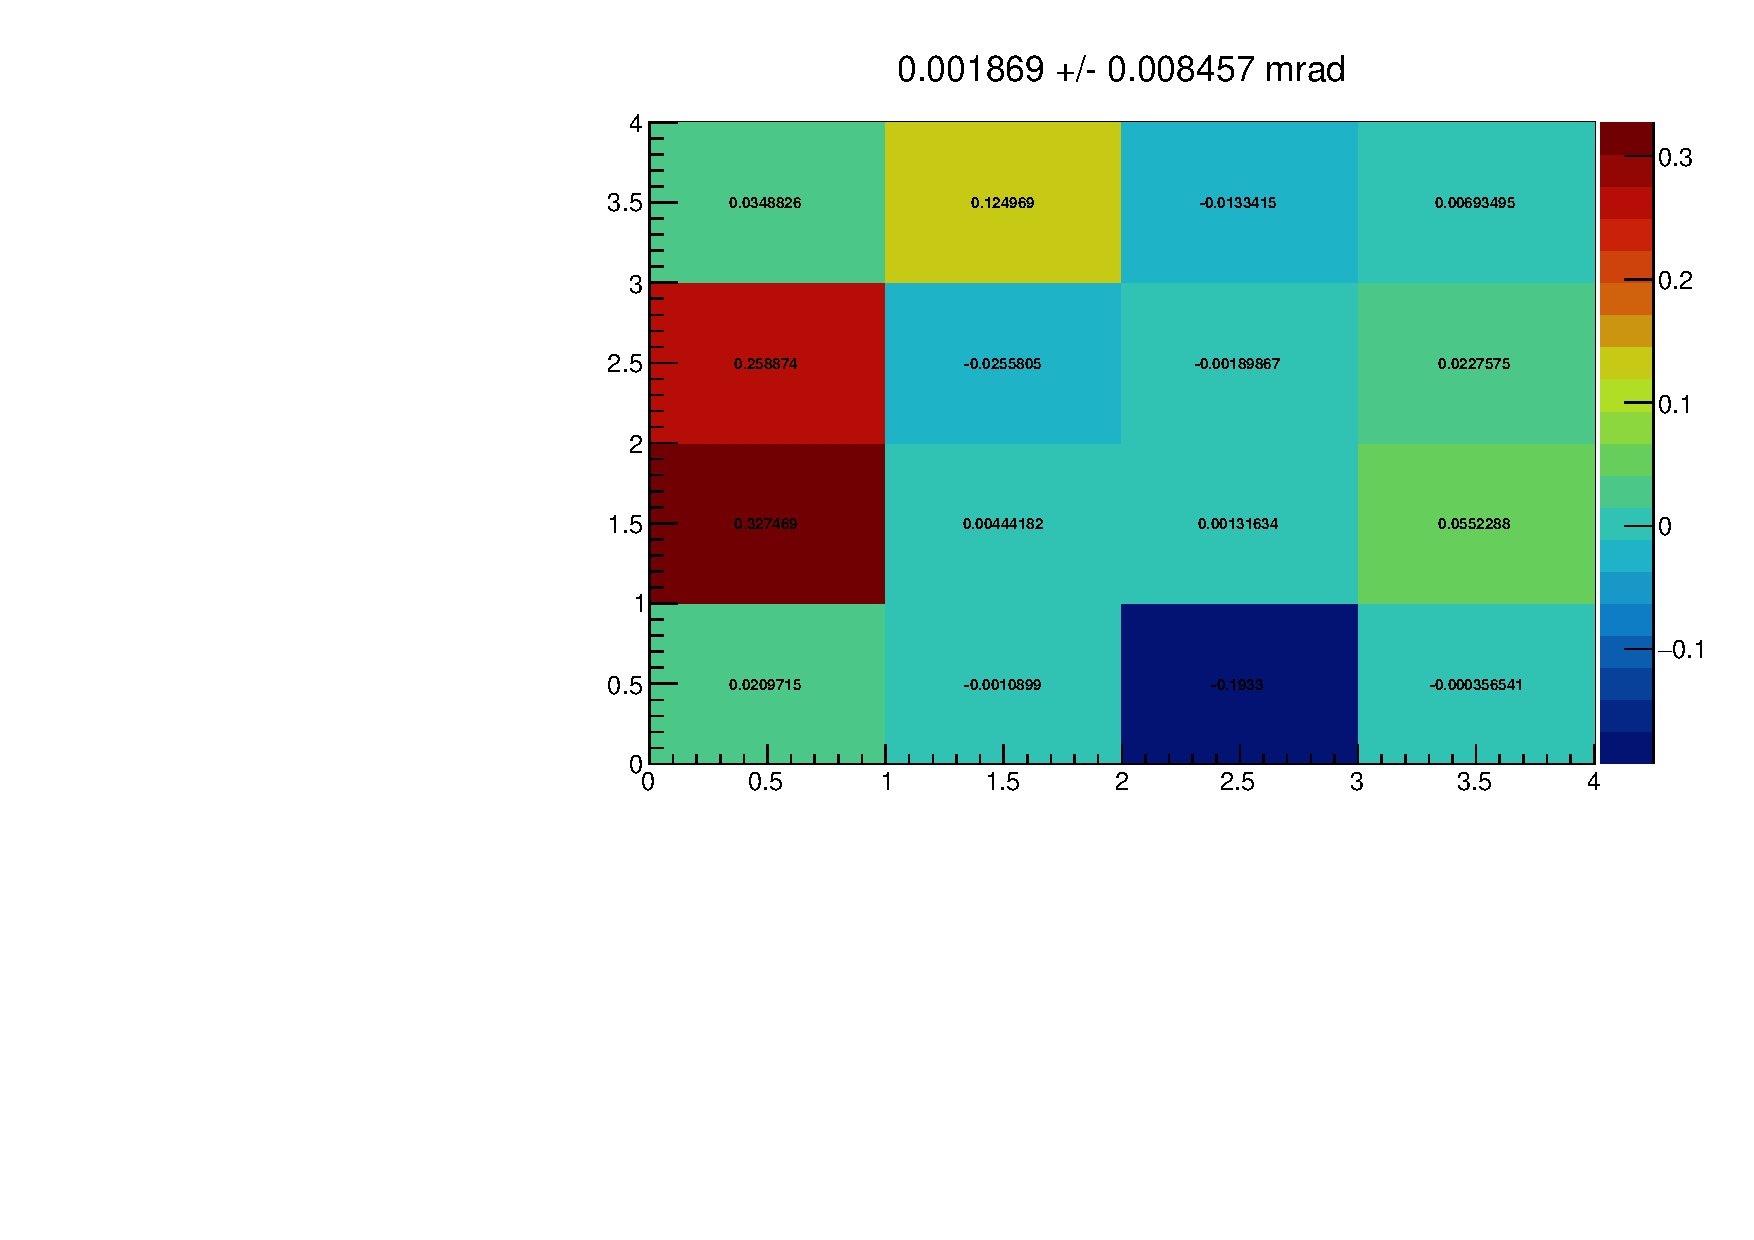
\includegraphics[width=0.48 \textwidth] {del_rich1_09092015.pdf}}
		\subfigure{ 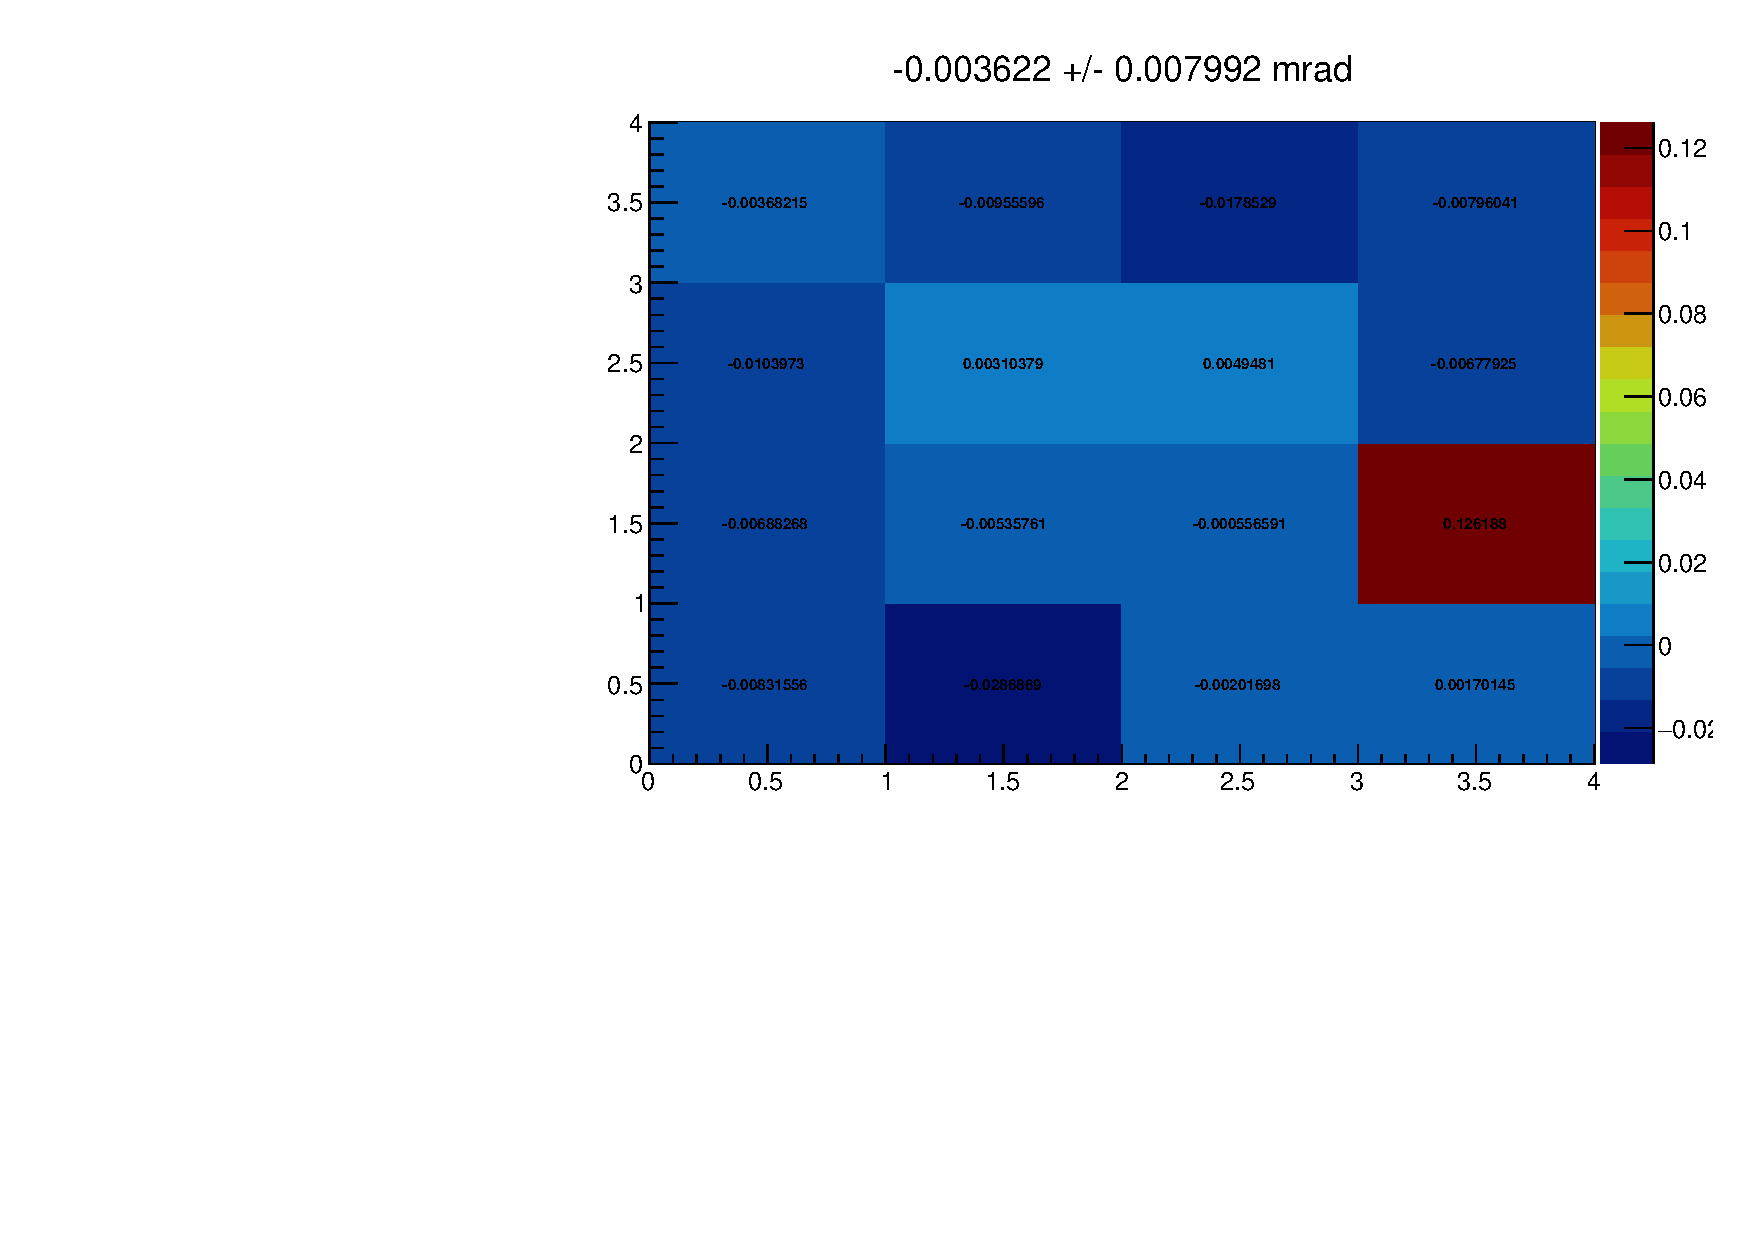
\includegraphics[width=0.48 \textwidth] {del_rich1_10092015.pdf}}
		\vspace*{-0.5cm}
	\end{center}
	\caption{\textit{Change in Cherenkov angle resolution for each mirror-pair in RICH1 in mrad between the first and the last iteration of three different alignments. Top left:} \textbf{first alignment}\textit{; top right:} \textbf{second alignment}\textit{; bottom:} \textbf{third alignment}\textit{. The value in the title of each plot is the absolute change Cherenkov angle resolution. } }
	\label{fig:rich1del}
\end{figure}

\subsubsection{Reference plot}
In order to quantify the above plots I compared the same alignment on different data samples. The alignment used was this made in the \textbf{second alignment}. It was applied to consecutive fills of mag up data. The resolution for each mirror-pair should be the same apart from statistical fluctuations due to different data-samples. The result is shown in Figure \ref{fig:rich1magup} and seem to show that fluctuations of $0.02\, mrad$ per mirror-pair and $0.001\, mrad$ overall can be purely due to statistics.\\
\begin{figure}[!h]
	\vspace*{-0.cm}
	\begin{center}
		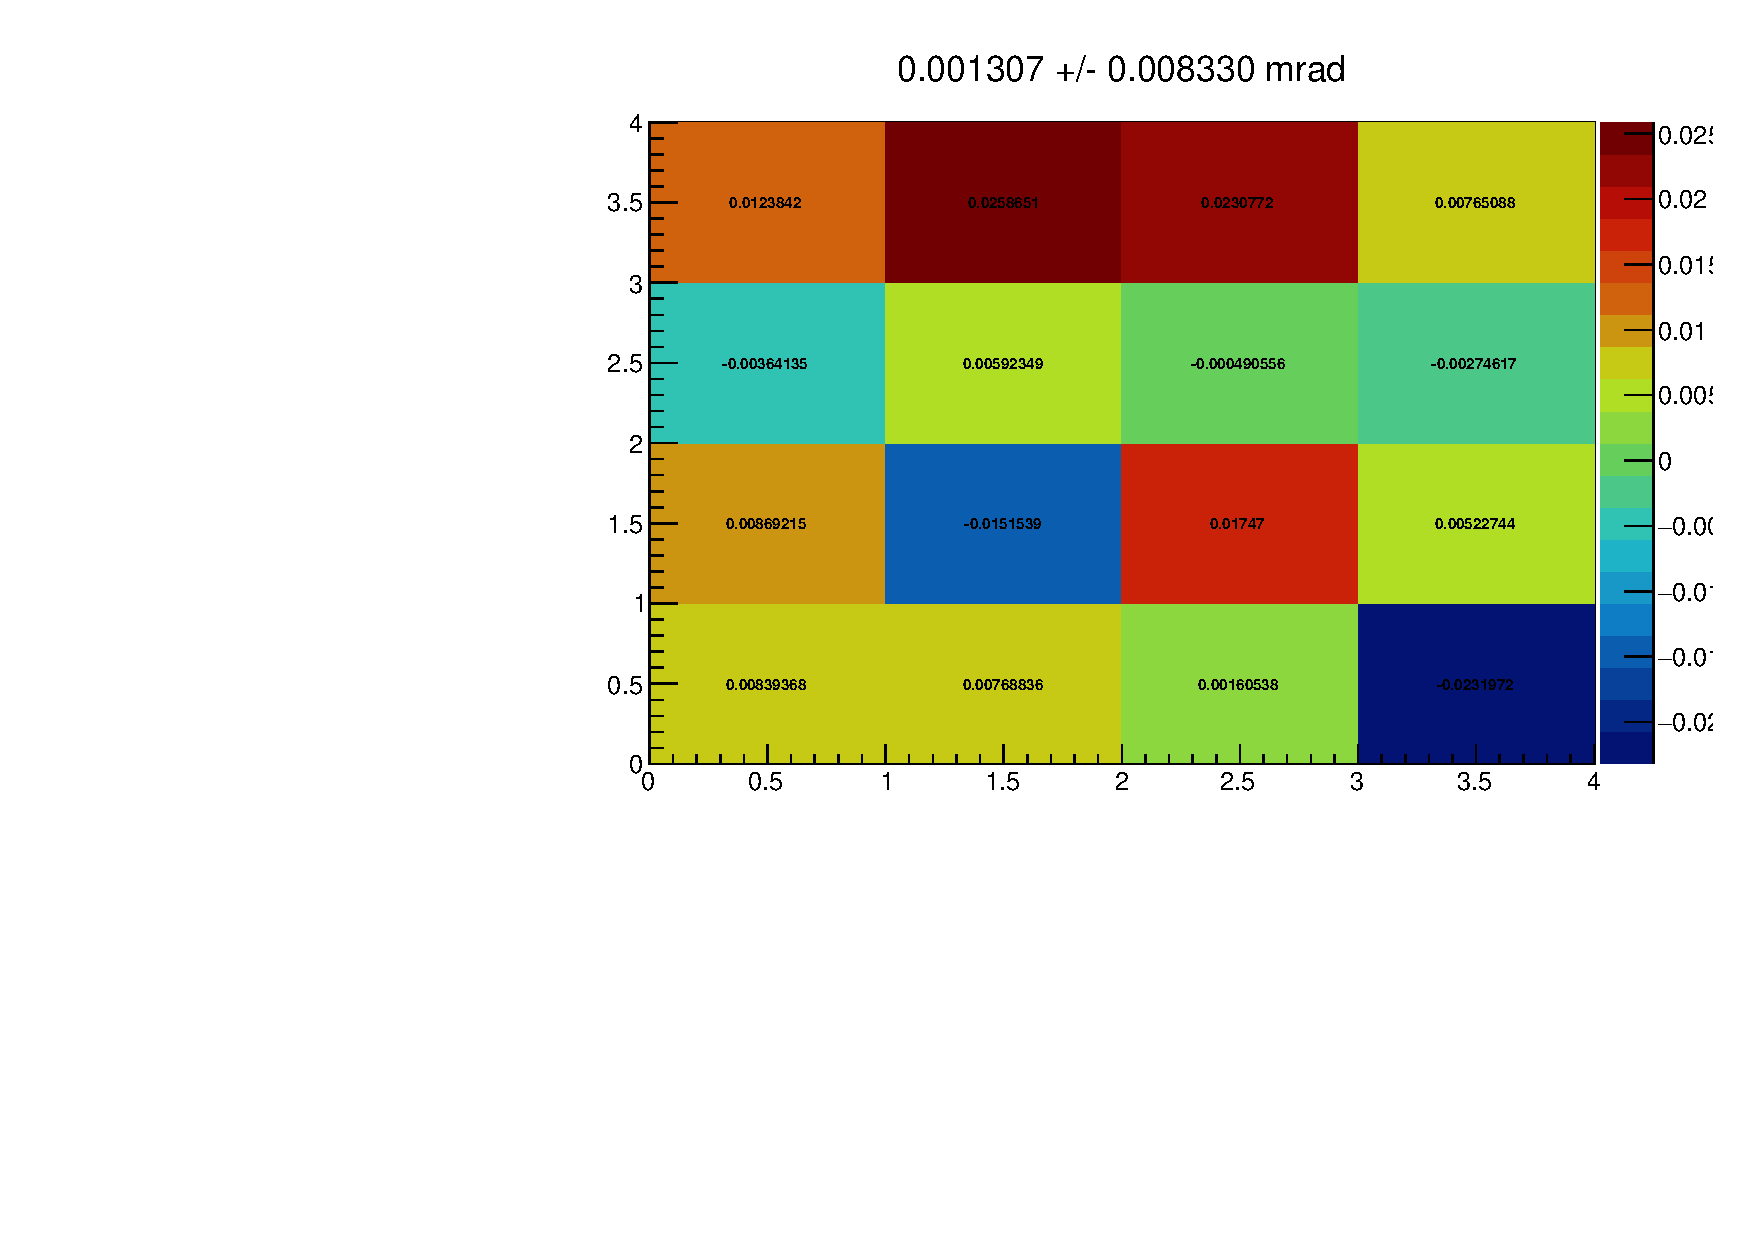
\includegraphics[width=0.7\textwidth]{del_rich1_magup.pdf}
		\vspace*{-0.5cm}
	\end{center}
	\caption{\textit{Difference in Cherenkov angle resolution for the same alignment applied to different data samples (consecutive fills of same polarity). }}
	\label{fig:rich1magup}
\end{figure}

Additionally the number of photon hits varies over the different mirror-pairs. This means that mirror-pairs with high population will contribute more to the total Cherenkov angle resolution than mirror-pairs with low population. The number of unambiguous photon hits per mirror-pair is shown below for the three alignments.\\
\begin{figure}[!h]
	\vspace*{-0.cm}
	\begin{center}
		\subfigure{ 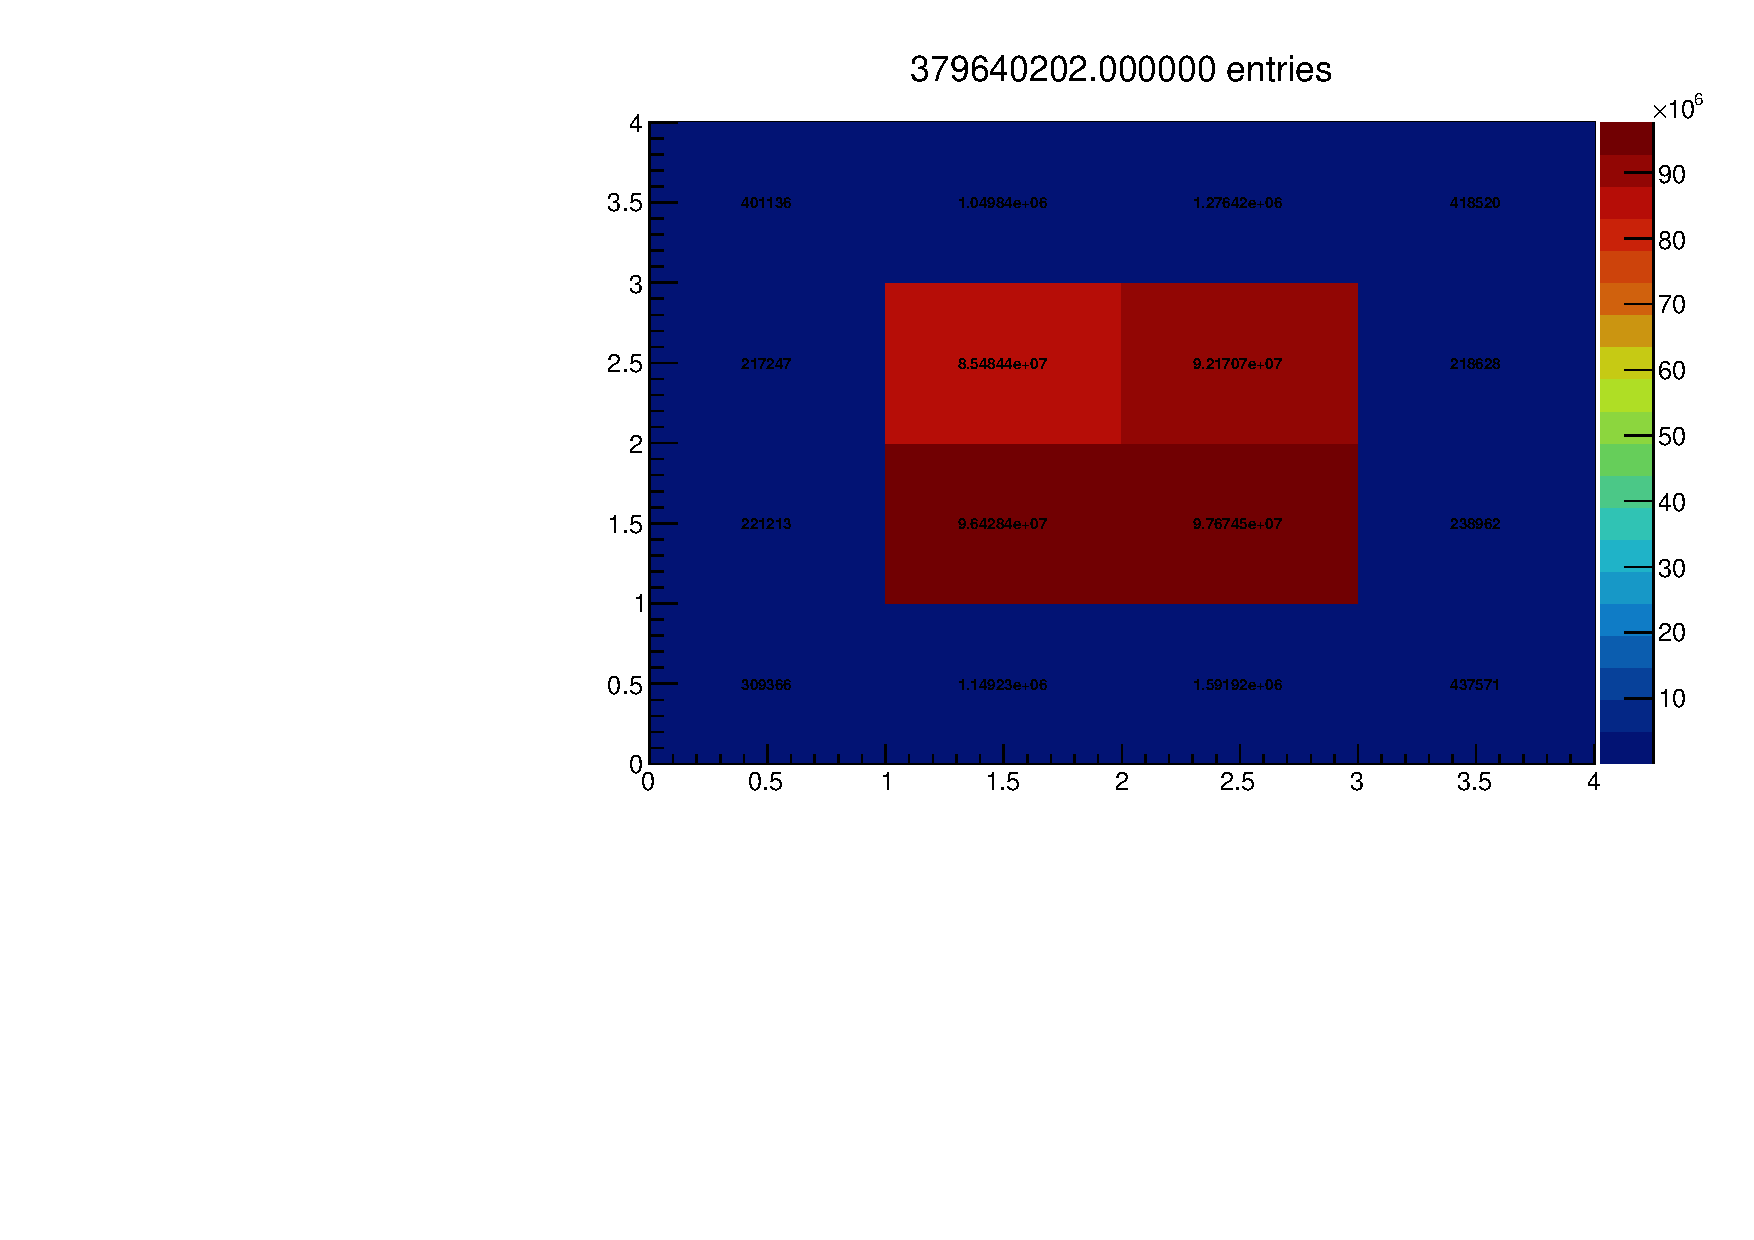
\includegraphics[width=0.48 \textwidth] {entries_rich1_11072015.pdf}}
		\subfigure{ 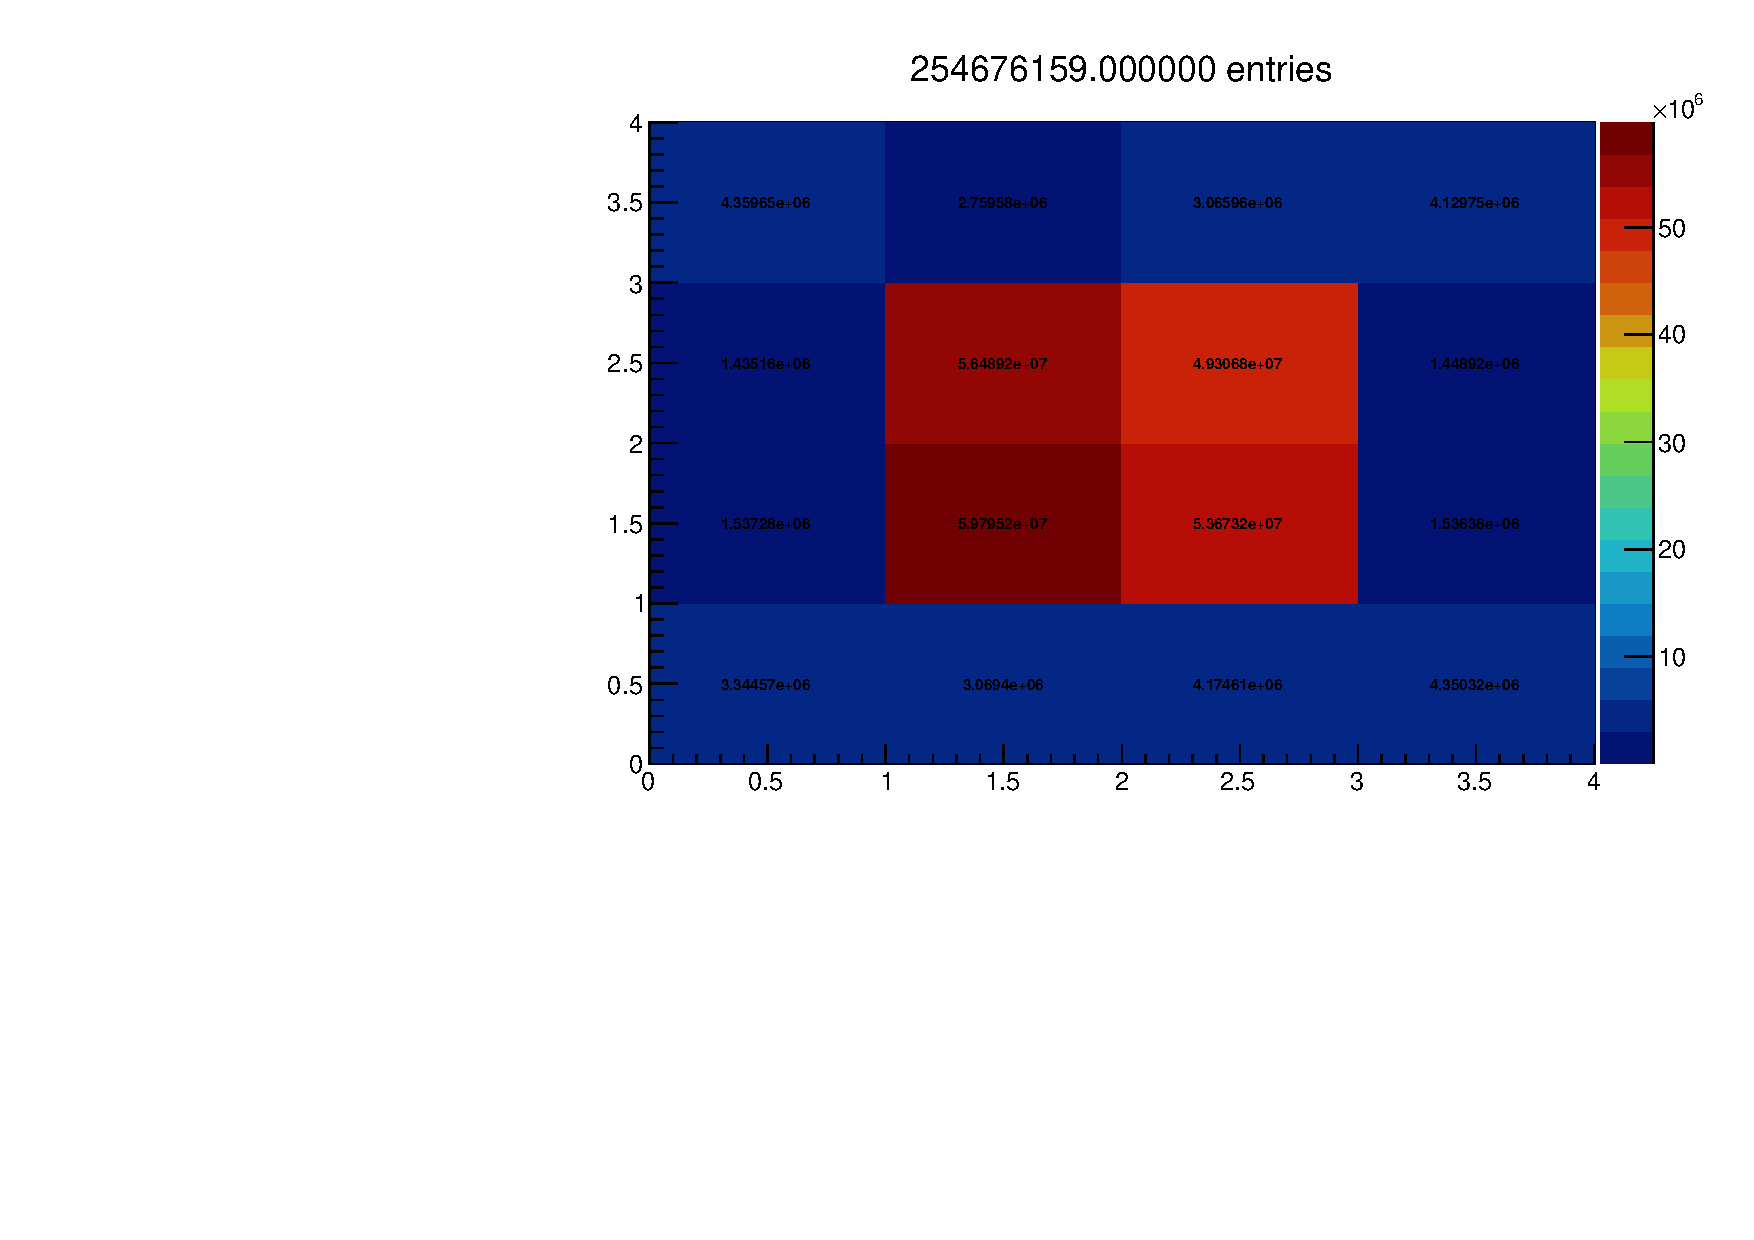
\includegraphics[width=0.48 \textwidth] {entries_rich1_09092015.pdf}}
		\subfigure{ 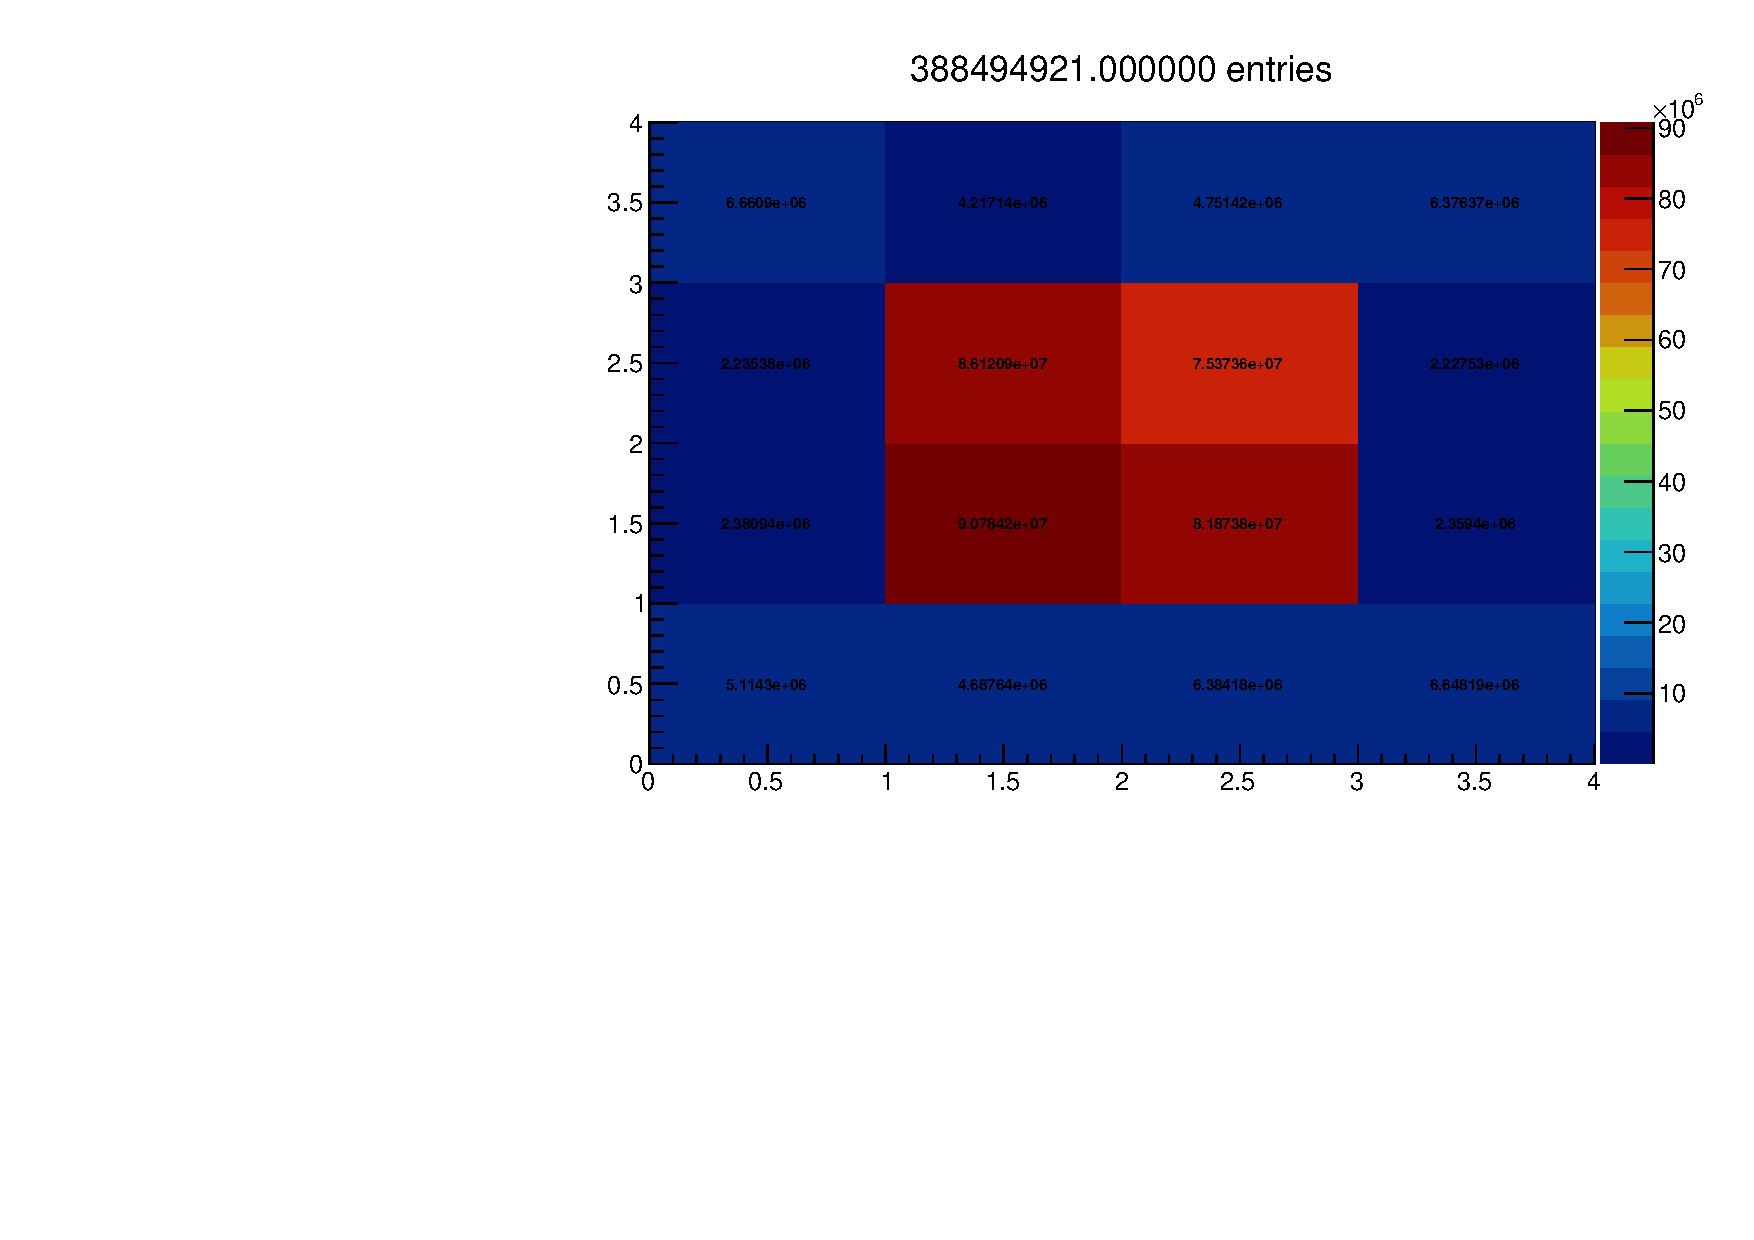
\includegraphics[width=0.48 \textwidth] {entries_rich1_10092015.pdf}}
		\vspace*{-0.5cm}
	\end{center}
	\caption{\textit{The number of unambiguous photon hits per mirror-pair for three different alignments. Top left:} \textbf{first alignment}\textit{; top right:} \textbf{second alignment}\textit{; bottom:} \textbf{third alignment}\textit{. The value in the title of each plot is the total number of unambiguous photons. } }
	\label{fig:rich1entries}
\end{figure}
Note that the RICH1 HLT line changed somewhere between the first and the second alignment.\\
\\

\clearpage





\section{RICH2}
\subsection{Introduction}
In RICH2 one given primary mirror can reflect onto several secondary mirrors and one given secondary mirror can receive photons from several primary mirrors. The primary and secondary mirrors of RICH2 are shown in Figure \ref{fig:rich2mirr}. The mirror-pairs for the left side of the RICH2 used in the alignment are shown in Figure \ref{fig:rich2combis}, the right side is equivalent. 
\begin{figure}[!h]
	\vspace*{-0.3cm}
	\begin{center}
		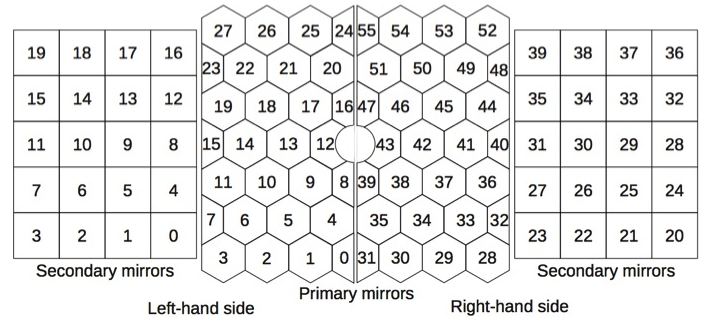
\includegraphics[width=1.\textwidth]{rich2mirrors.png}
		\vspace*{-1.cm}
	\end{center}
	\caption{\textit{Primary and secondary mirrors of RICH2.}}
	\label{fig:rich2mirr}
\end{figure}

\begin{figure}[!h]
	\vspace*{-0.4cm}
	\begin{center}
		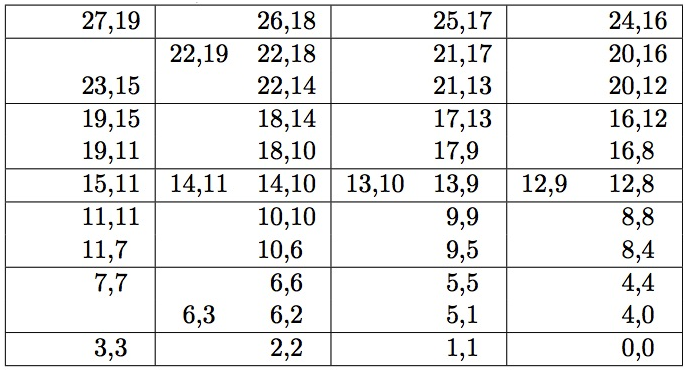
\includegraphics[width=0.7\textwidth]{rich2combis.png}
		\vspace*{-0.5cm}
	\end{center}
	\caption{\textit{Mirror combinations of the left side of RICH2 used in the alignment procedure.}}
	\label{fig:rich2combis}
\end{figure}

Mirror pairs are denoted by a four-digit number where the first two numbers refer to the primary mirror and the last two to the secondary mirror.\\
\\
In the following different quantities are compared by mirror-pair. In order to make the information as accessible as possible the values will be shown in heatmaps where each bin will represent a mirror pair. For RICH2 the bins are the schematic position of the mirror-pairs as shown in Figure \ref{fig:rich2combis}.
\\
\clearpage
\subsection{Cherenkov angle resolution by mirror-pair}
Here the Cherenkov angle resolution for each mirror-pair is shown for three different alignments which actually converged. \\
The \textbf{first alignment} is the very first alignment made on 2015 data that converged. It was made offline on the very first data taken (mag down). It started from a 2012 alignment that did not use the new MDCS. This alignment converged after 5 iterations and was initially used in the database.\\
The \textbf{second alignment} was made online with early measurement data on the 19.07.2015 and is currently being used in the database. It converged after 4 iterations.\\
The \textbf{third alignment} was made on three fills of mag up data on the 09.09.2015. The alignment procedure started with the second alignment and converged after 2 iterations.\\
Note that these alignments differ from those used for RICH1. Basically the first alignment for RICH1 corresponds to the second one for RICH2 while the second alignment for RICH1 corresponds to the third for RICH2.\\
Figure \ref{fig:rich2maps} shows the Cherenkov angle resolution at the end of each alignment for each mirror pair in $mrad$. The value in the title of each plot is the absolute Cherenkov angle resolution.
\begin{figure}[!h]
	\vspace*{-0.cm}
	\begin{center}
		\subfigure{ 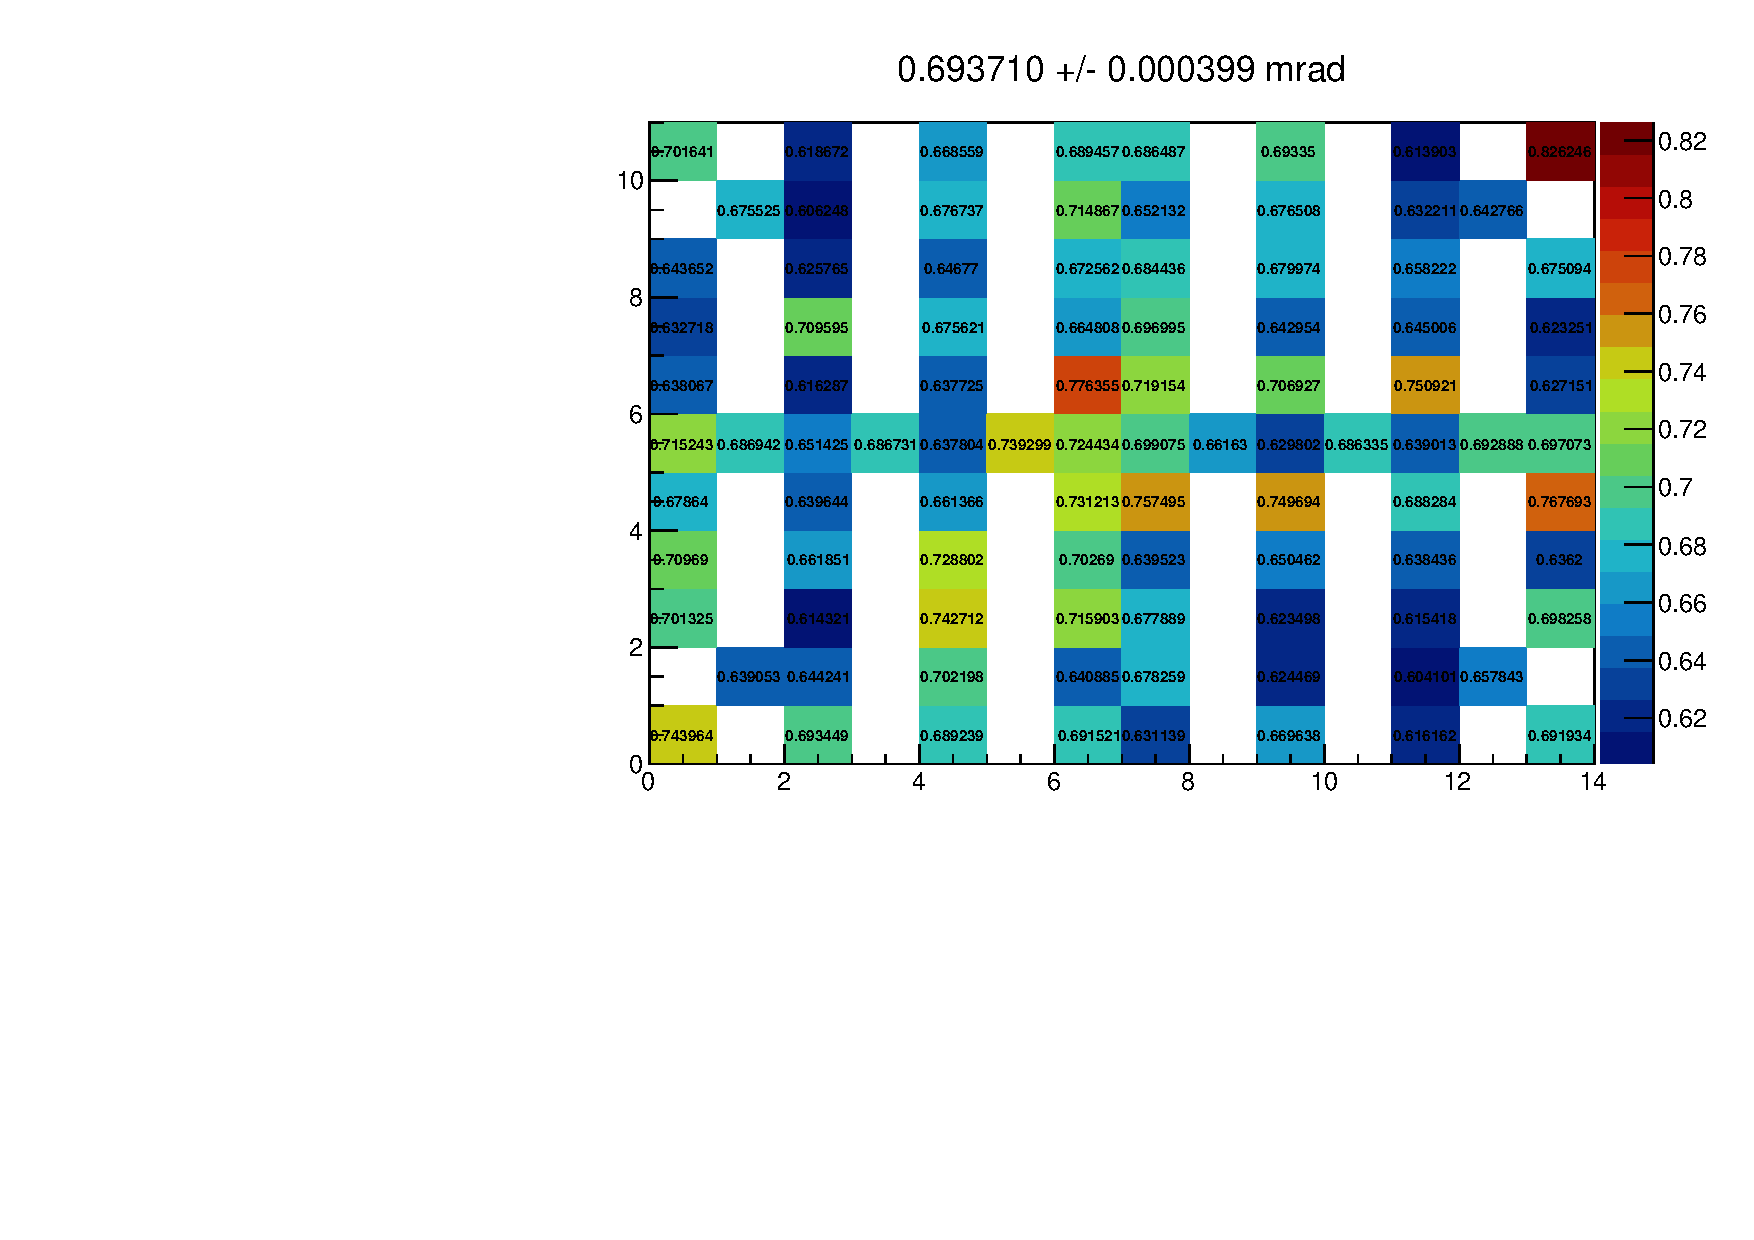
\includegraphics[width=0.48 \textwidth] {map_rich2_2015MDCS.pdf}}
		\subfigure{ 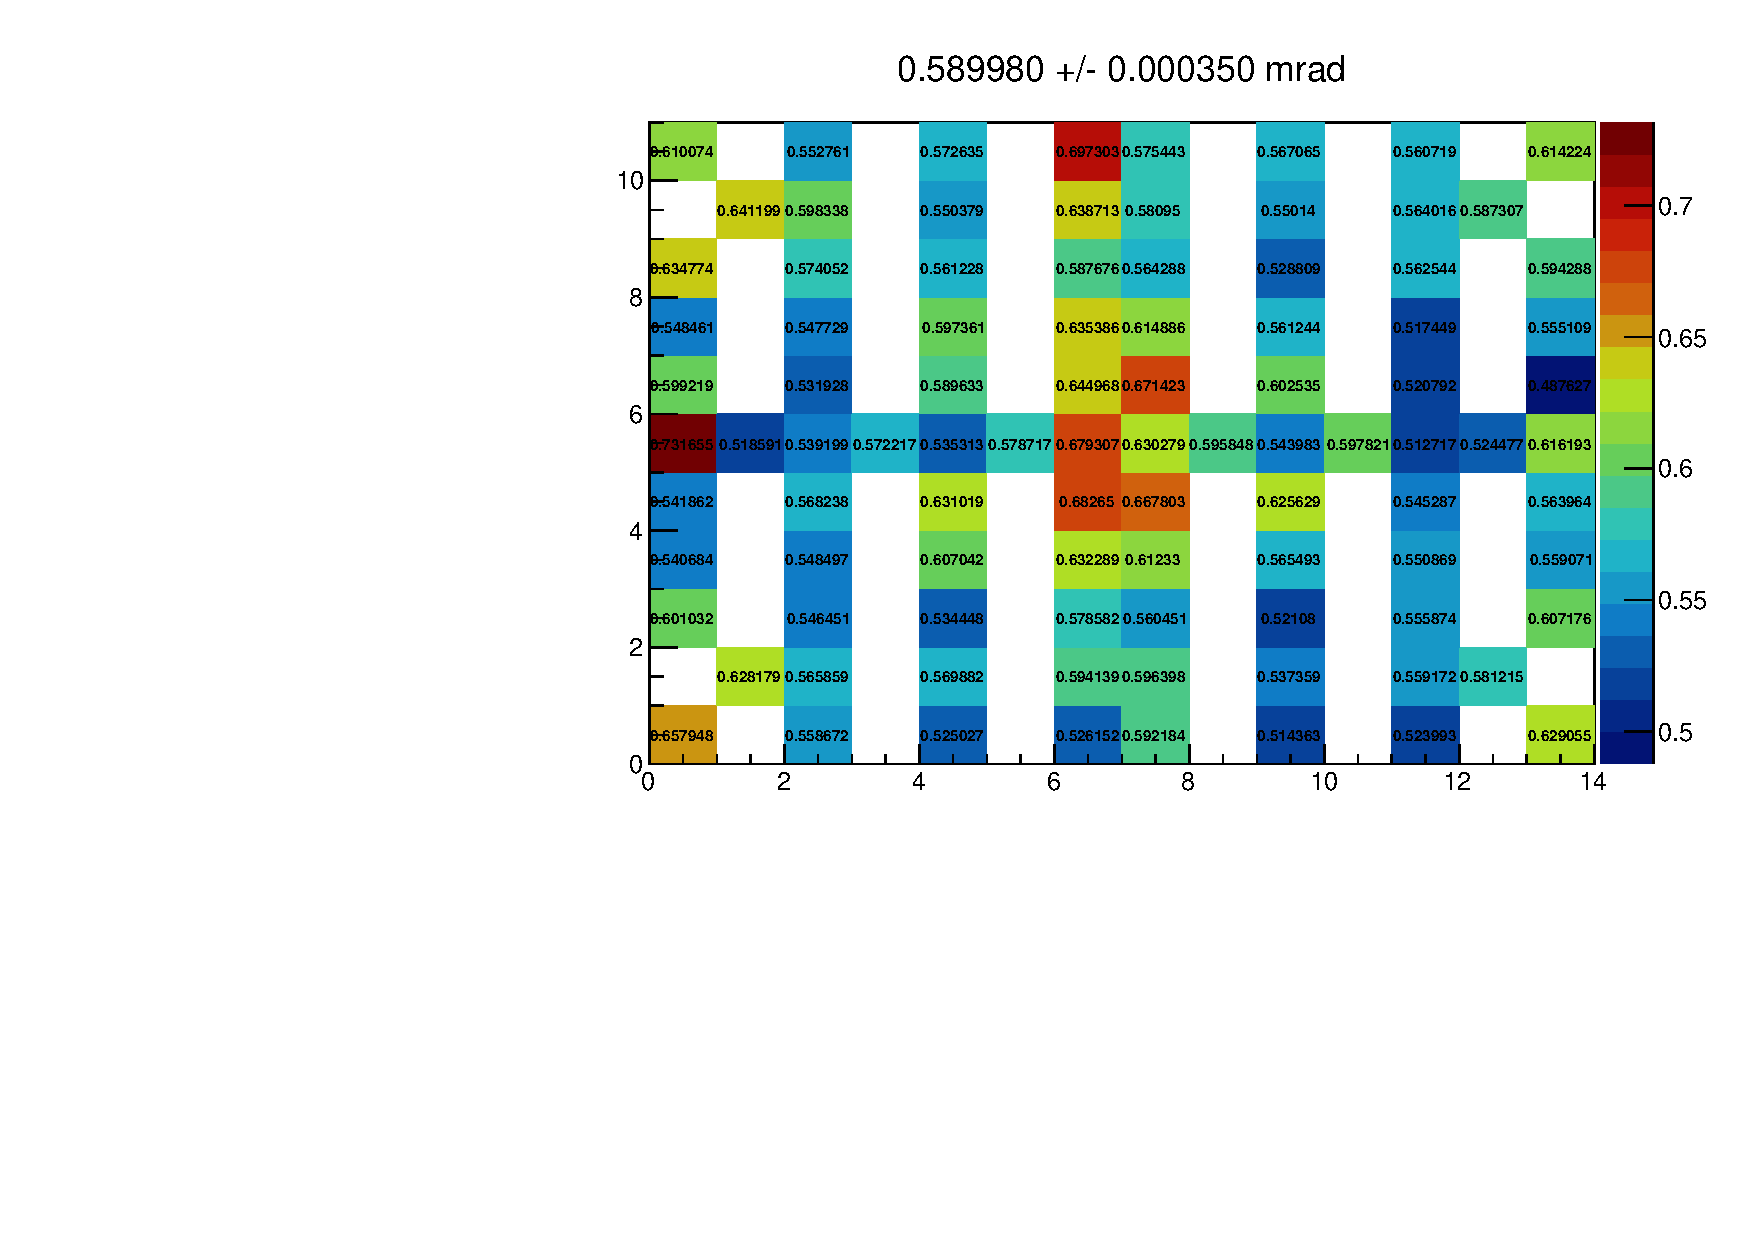
\includegraphics[width=0.48 \textwidth] {map_rich2_19072015.pdf}}
		\subfigure{ 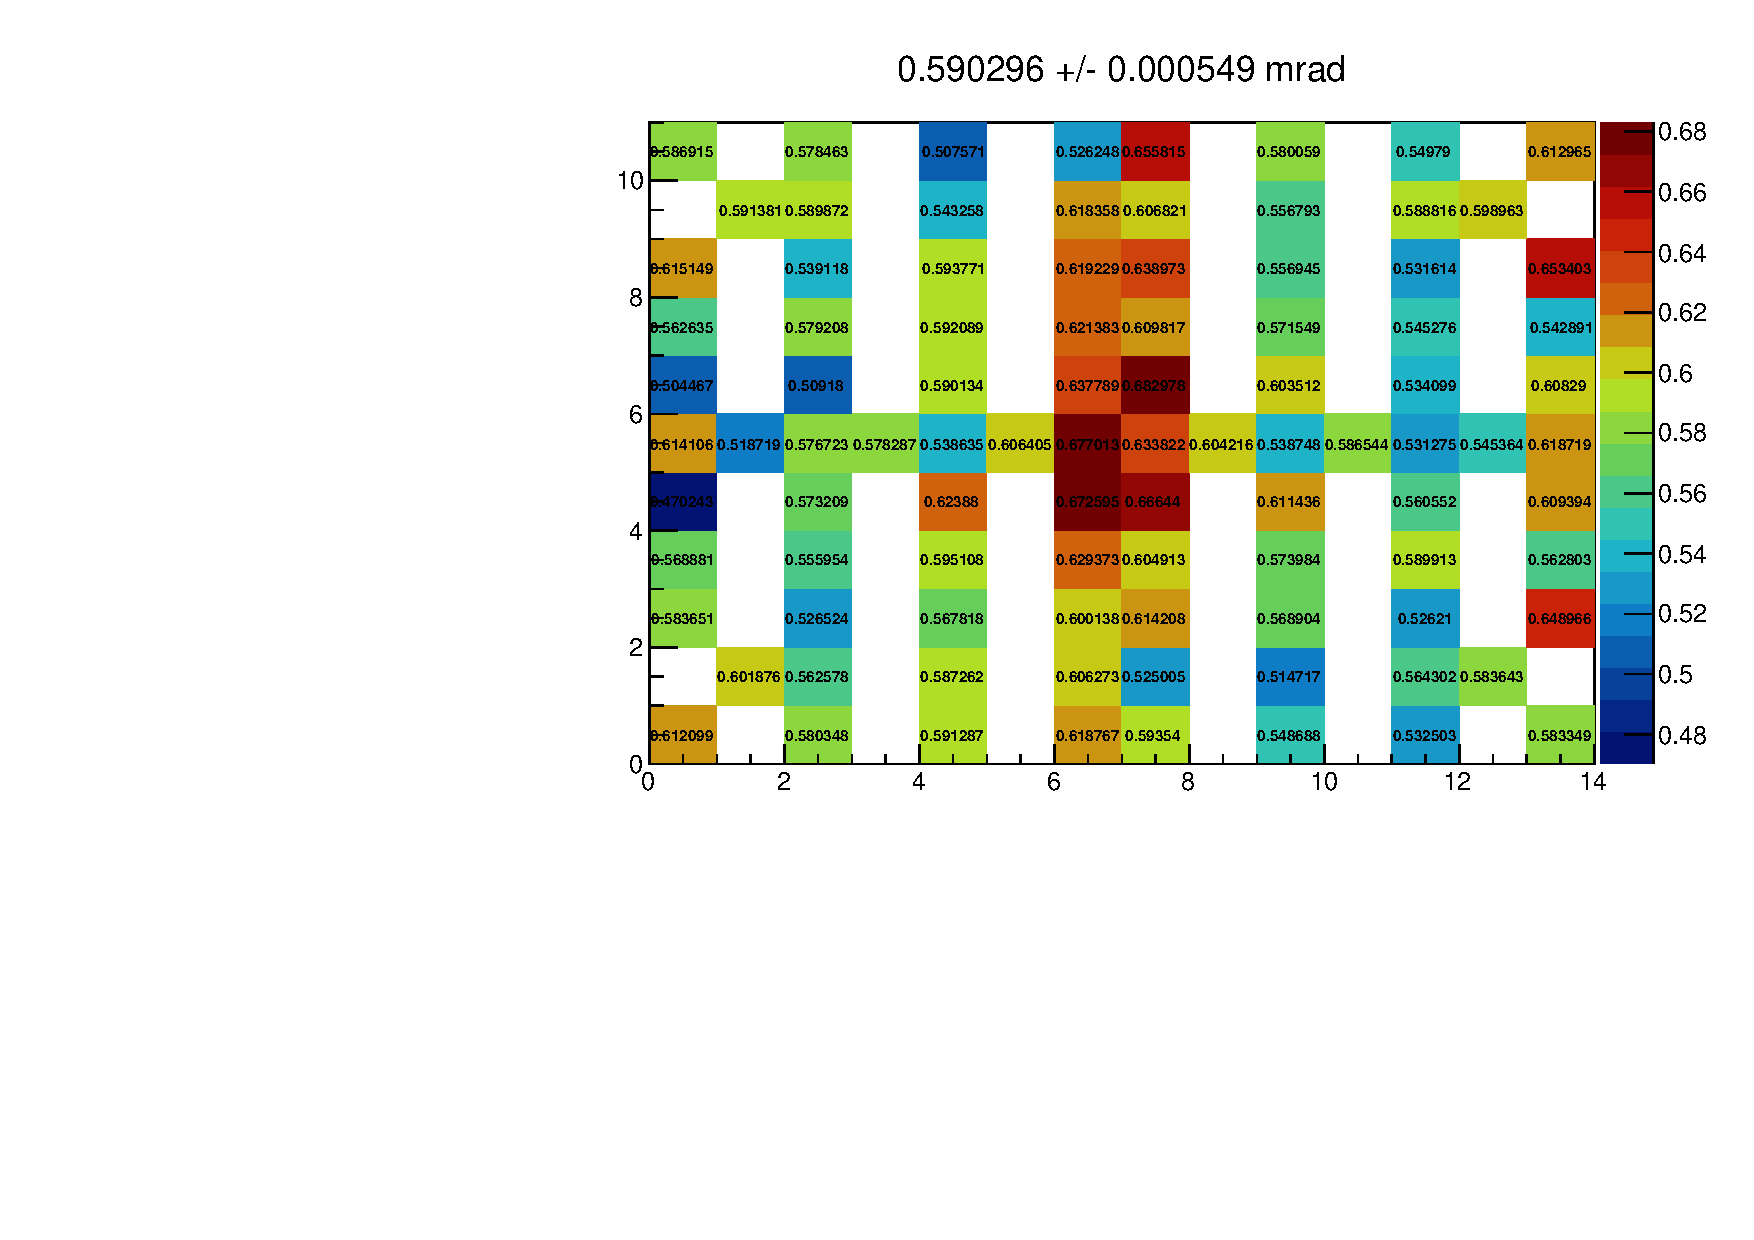
\includegraphics[width=0.48 \textwidth] {map_rich2_09092015.pdf}}
		\vspace*{-0.5cm}
	\end{center}
	\caption{\textit{Cherenkov angle resolution for each mirror-pair in RICH2 in mrad. Top left:} \textbf{first alignment}\textit{; top right:} \textbf{second alignment}\textit{; bottom:} \textbf{third alignment}\textit{. The value in the title of each plot is the absolute Cherenkov angle resolution. } }
	\label{fig:rich2maps}
\end{figure}


\subsection{Change of Cherenkov angle resolution over alignment}
Here the change of the Cherenkov angle resolution between the first and the last iteration of the above three alignments is shown.\\
Figure \ref{fig:rich2del} shows the change in Cherenkov angle resolution for each mirror pair in $mrad$. The value in the title of each plot is the absolute change in Cherenkov angle resolution.\\
\begin{figure}[!h]
	\vspace*{-0.cm}
	\begin{center}
		\subfigure{ 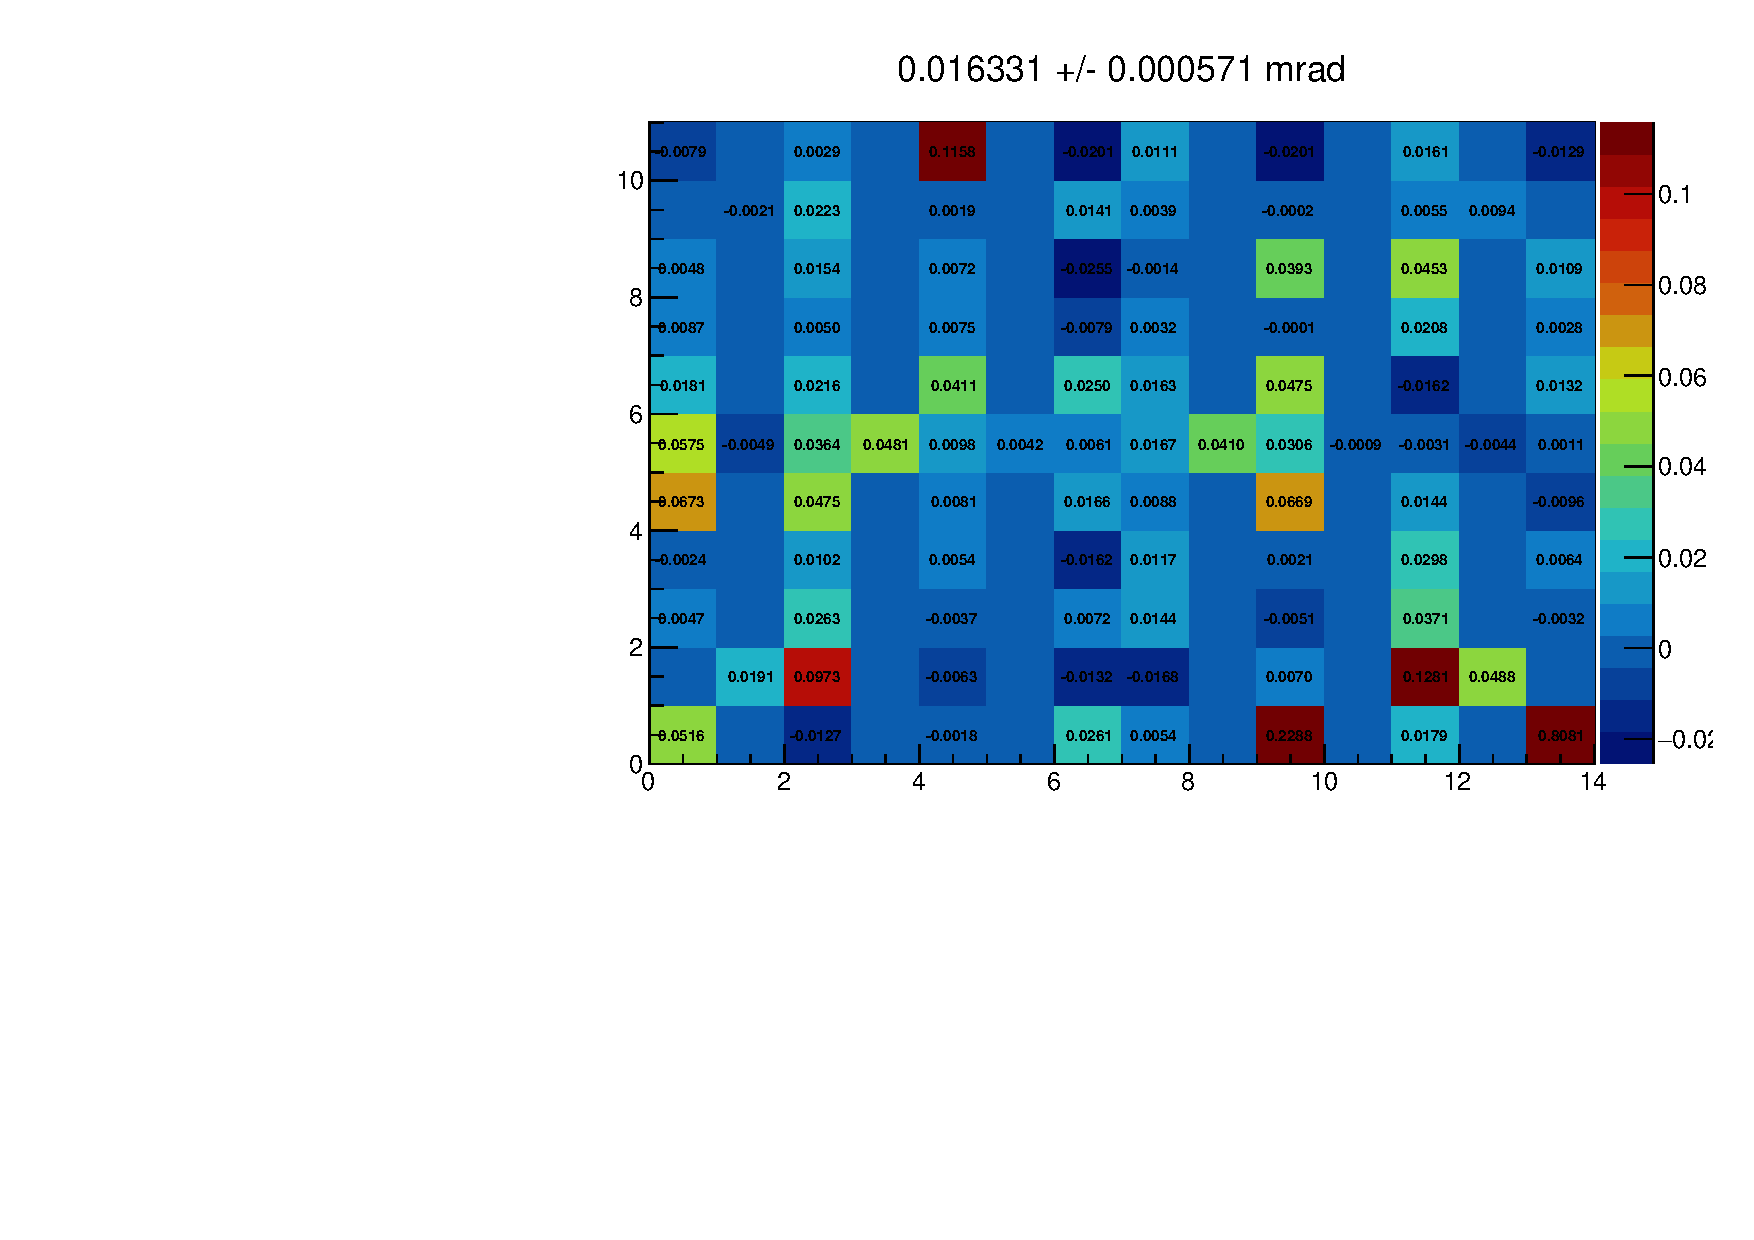
\includegraphics[width=0.48 \textwidth] {del_rich2_2015MDCS.pdf}}
		\subfigure{ 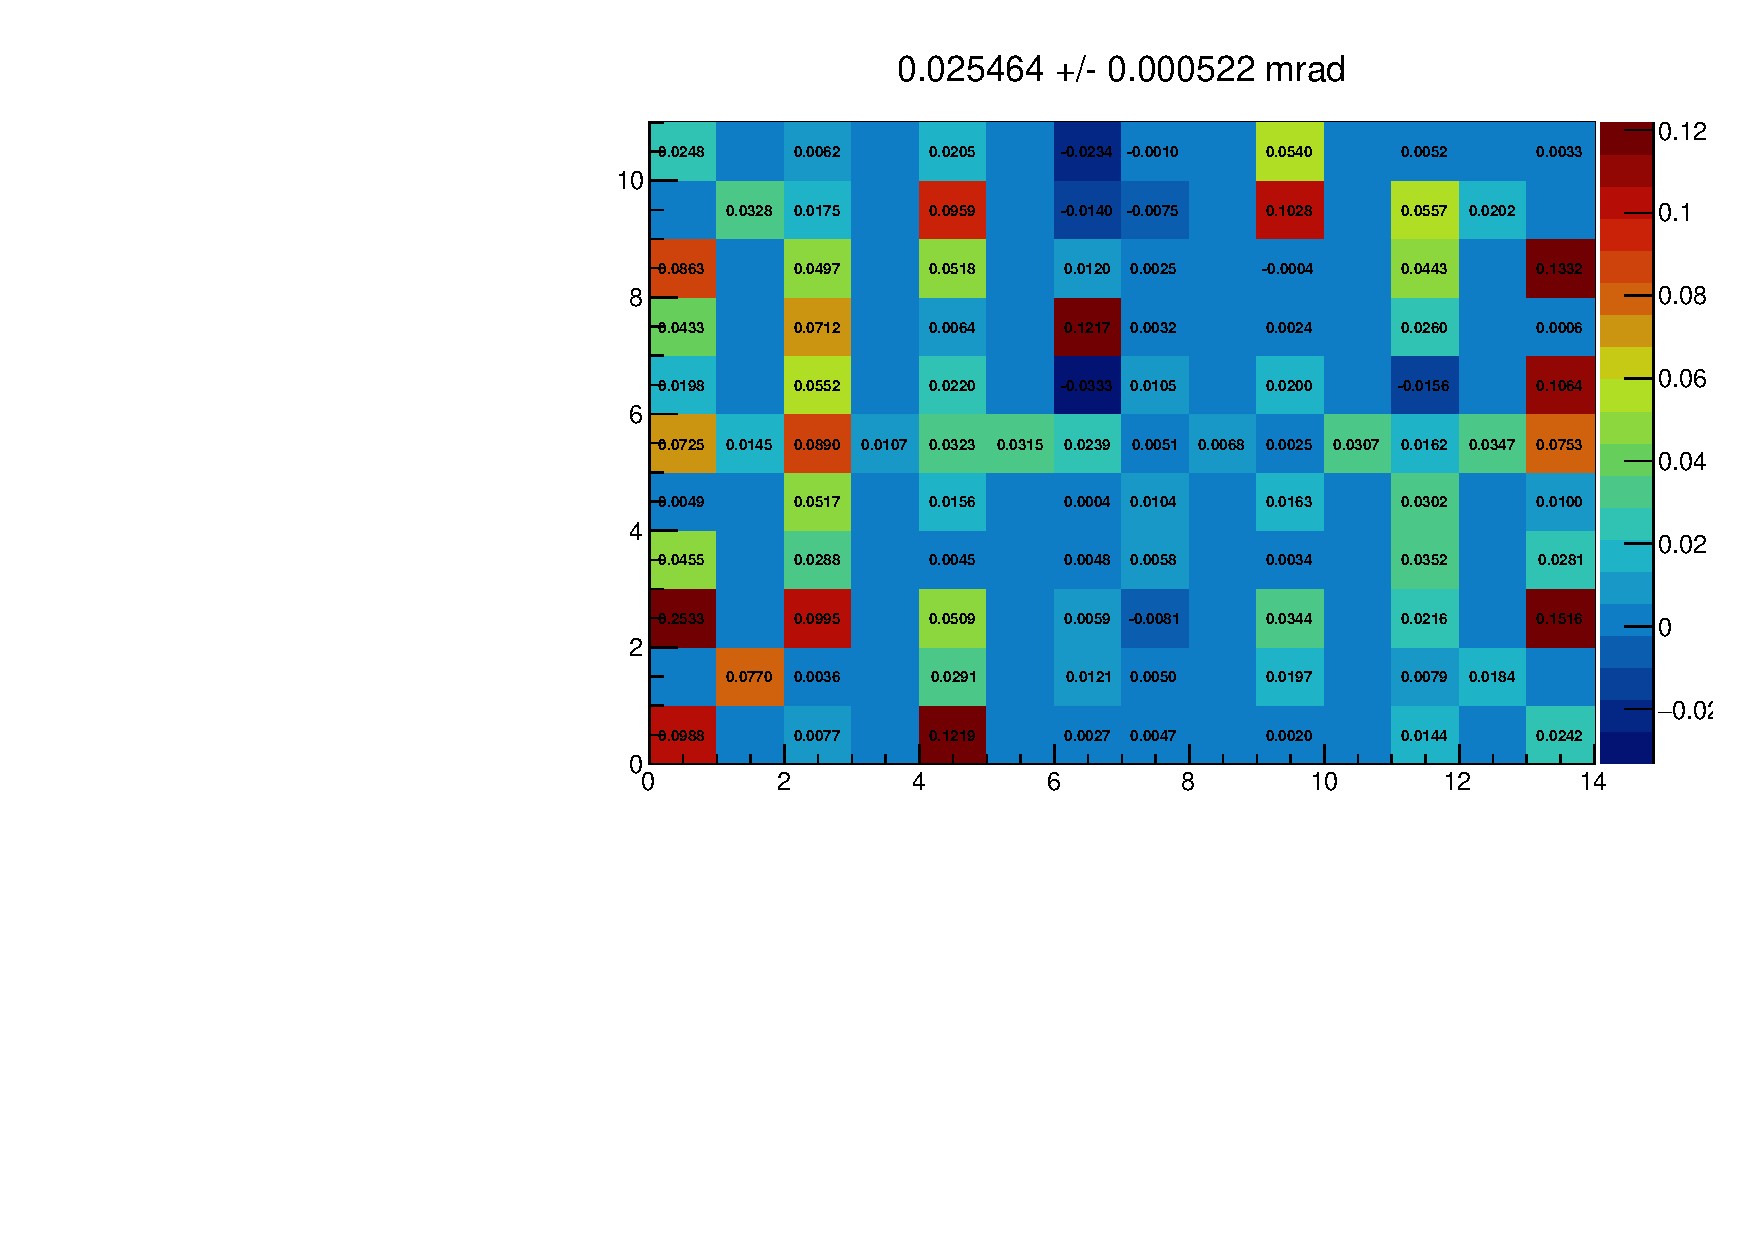
\includegraphics[width=0.48 \textwidth] {del_rich2_19072015.pdf}}
		\subfigure{ 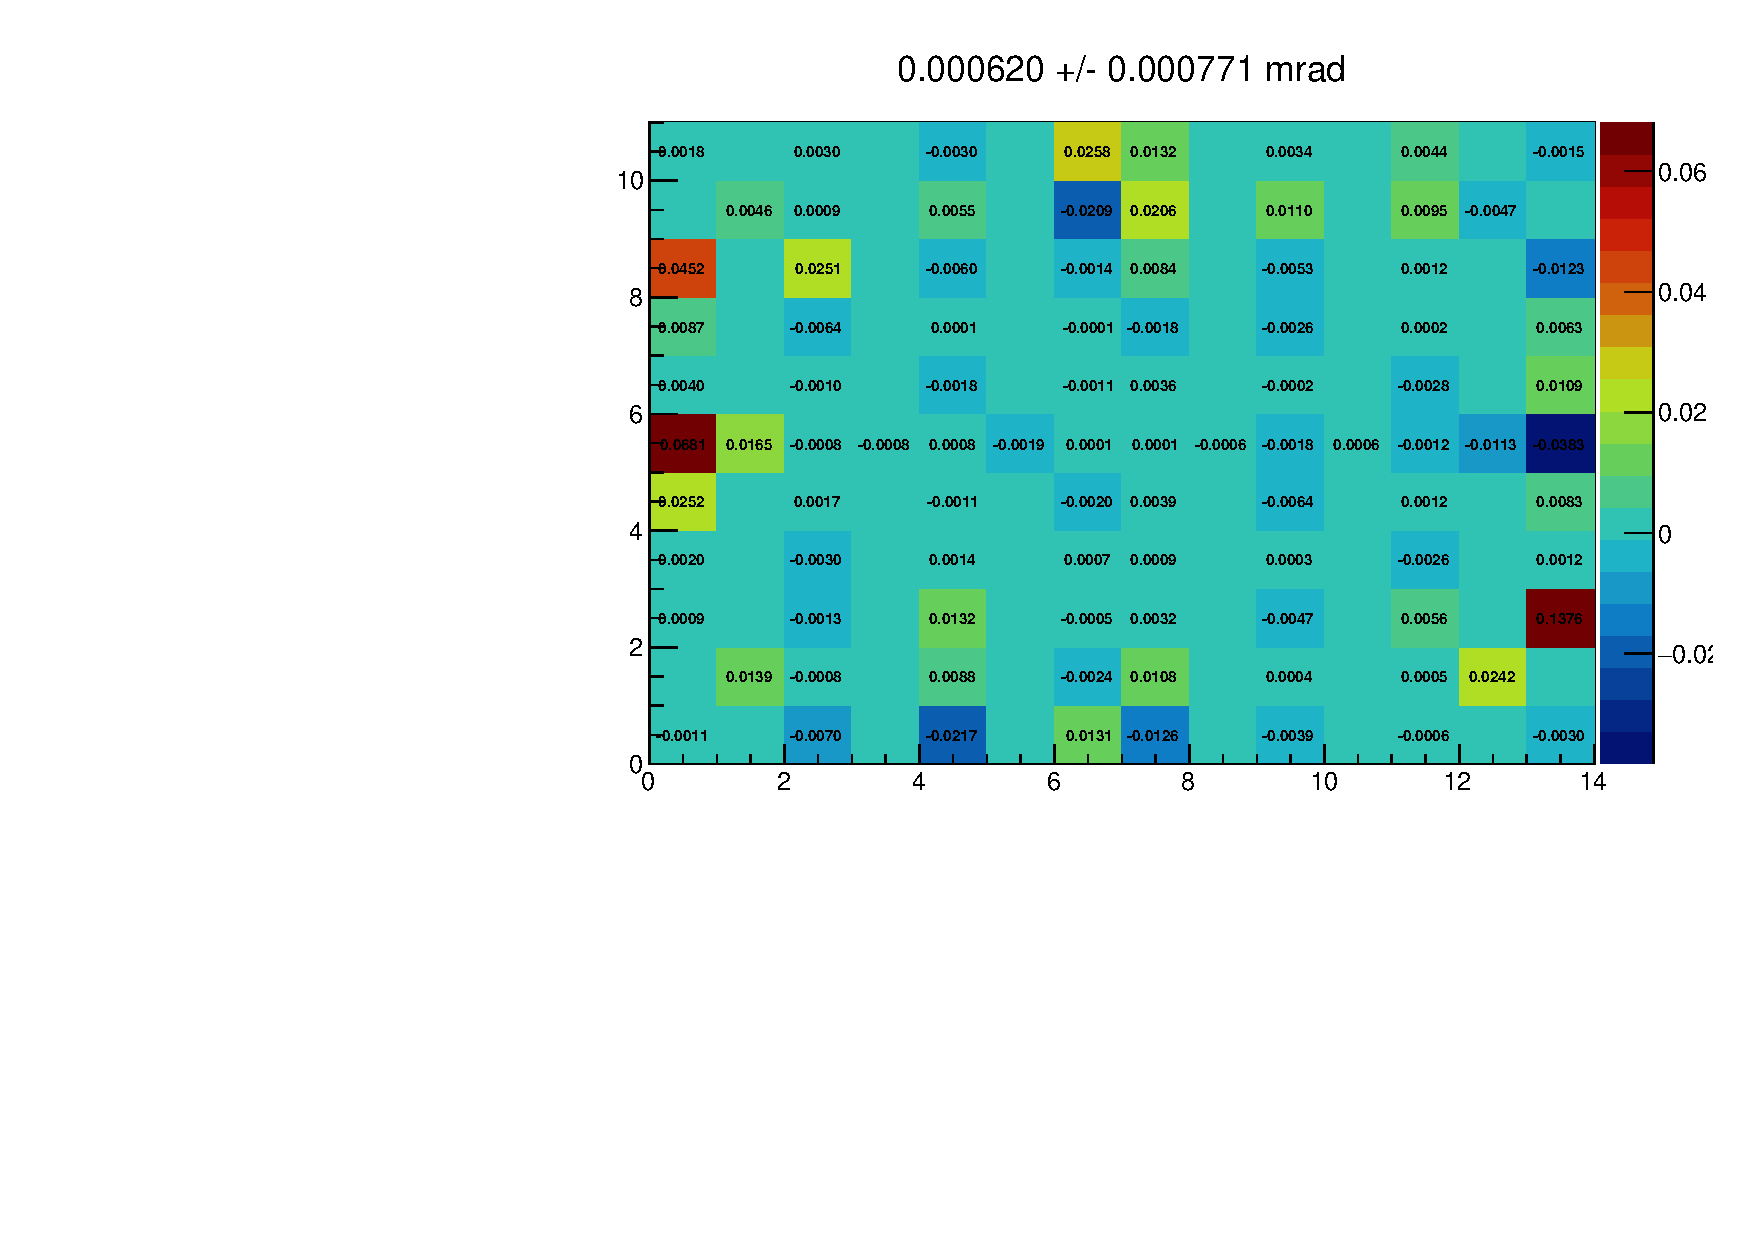
\includegraphics[width=0.48 \textwidth] {del_rich2_09092015.pdf}}
		\vspace*{-0.5cm}
	\end{center}
	\caption{\textit{Change in Cherenkov angle resolution for each mirror-pair in RICH2 in mrad between the first and the last iteration of three different alignments. Top left:} \textbf{first alignment}\textit{; top right:} \textbf{second alignment}\textit{; bottom:} \textbf{third alignment}\textit{. The value in the title of each plot is the absolute change Cherenkov angle resolution. } }
	\label{fig:rich2del}
\end{figure}
Note that for each alignment one fit failed and gave a too big number. This number was ignored when setting the limits on the z-axis.\\

\subsubsection{Reference plot}
Unfortunately no reference plots exists for RICH2 since there has not been enough alignment-farm time (yet).\\
\\
The number of photon hits varies over the different mirror-pairs. This means that mirror-pairs with high population will contribute more to the total Cherenkov angle resolution than mirror-pairs with low population. The number of unambiguous photon hits per mirror-pair is shown below for the three alignments.\\
\begin{figure}[!h]
	\vspace*{-0.cm}
	\begin{center}
		\subfigure{ 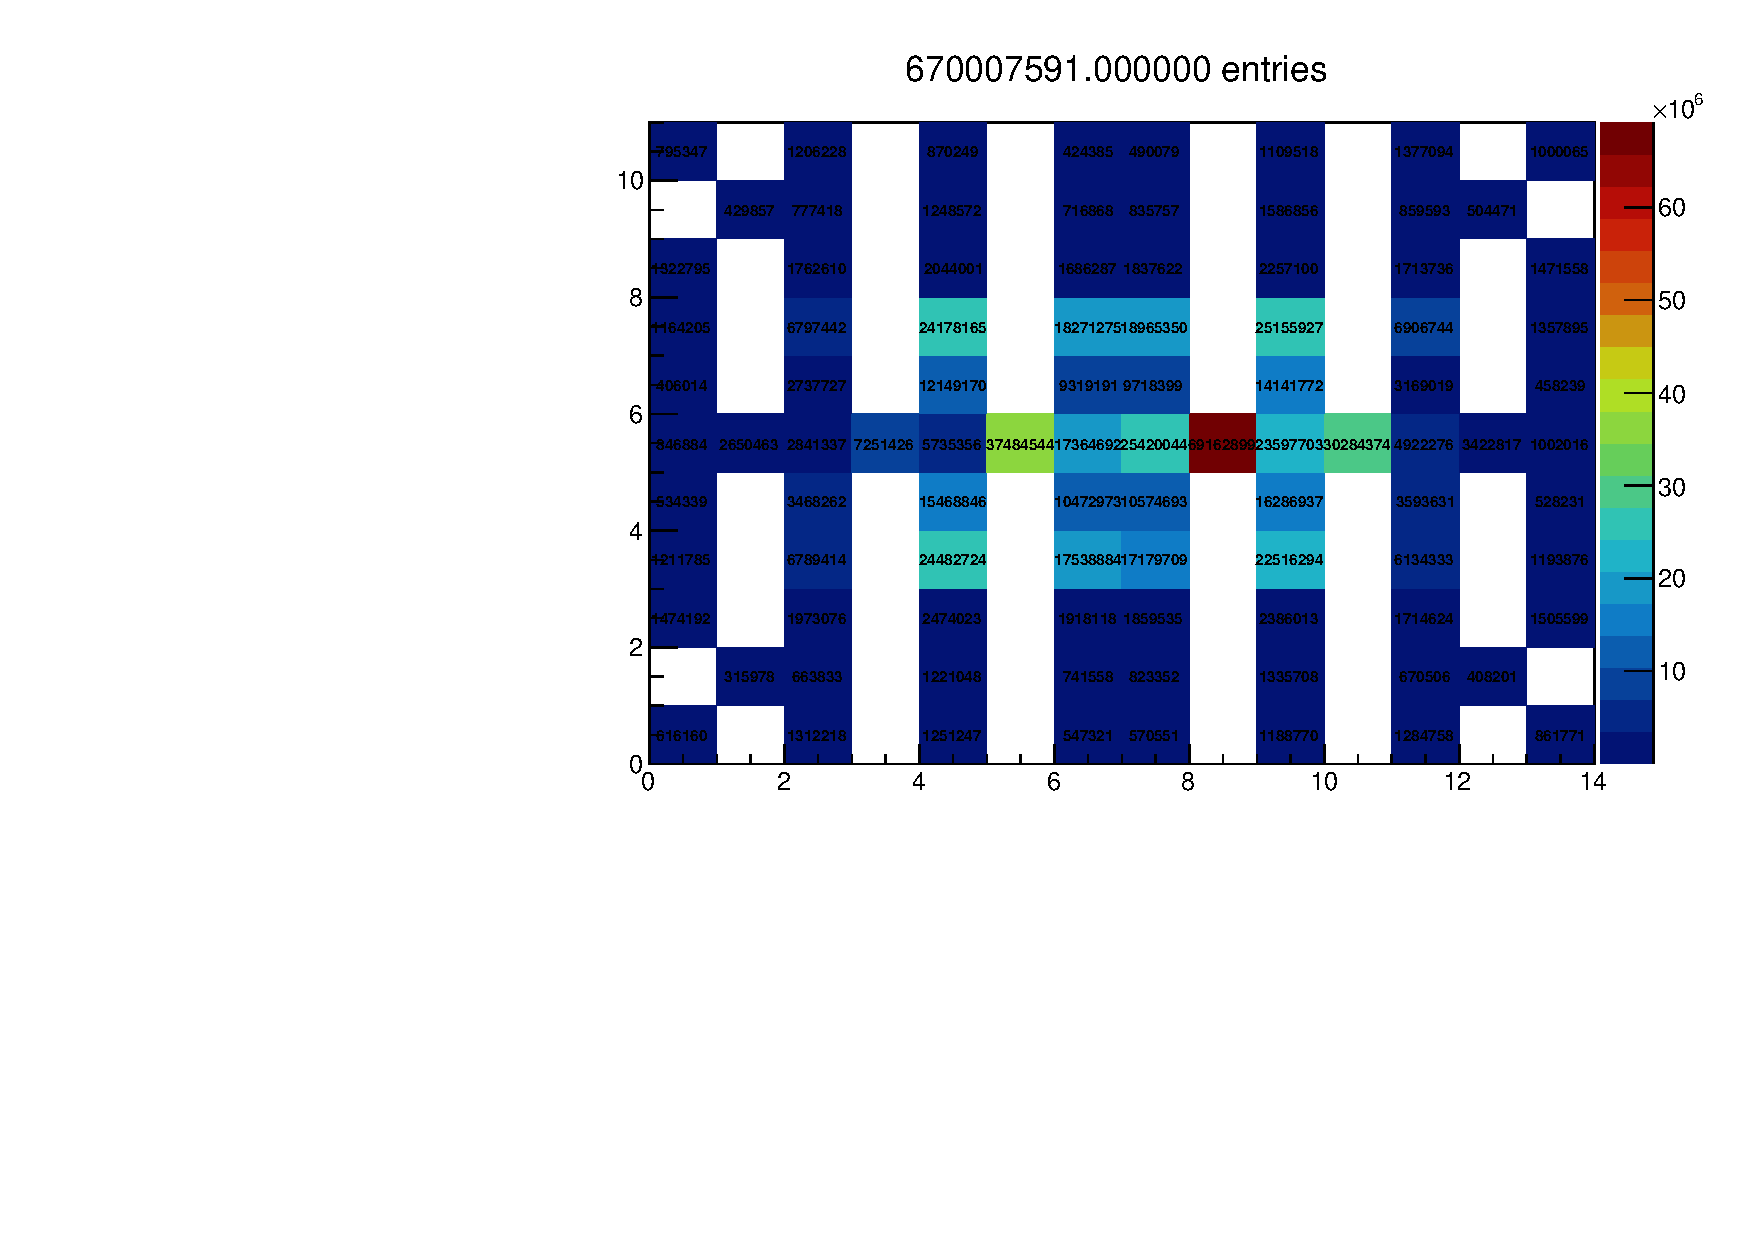
\includegraphics[width=0.48 \textwidth] {entries_rich2_2015MDCS.pdf}}
		\subfigure{ 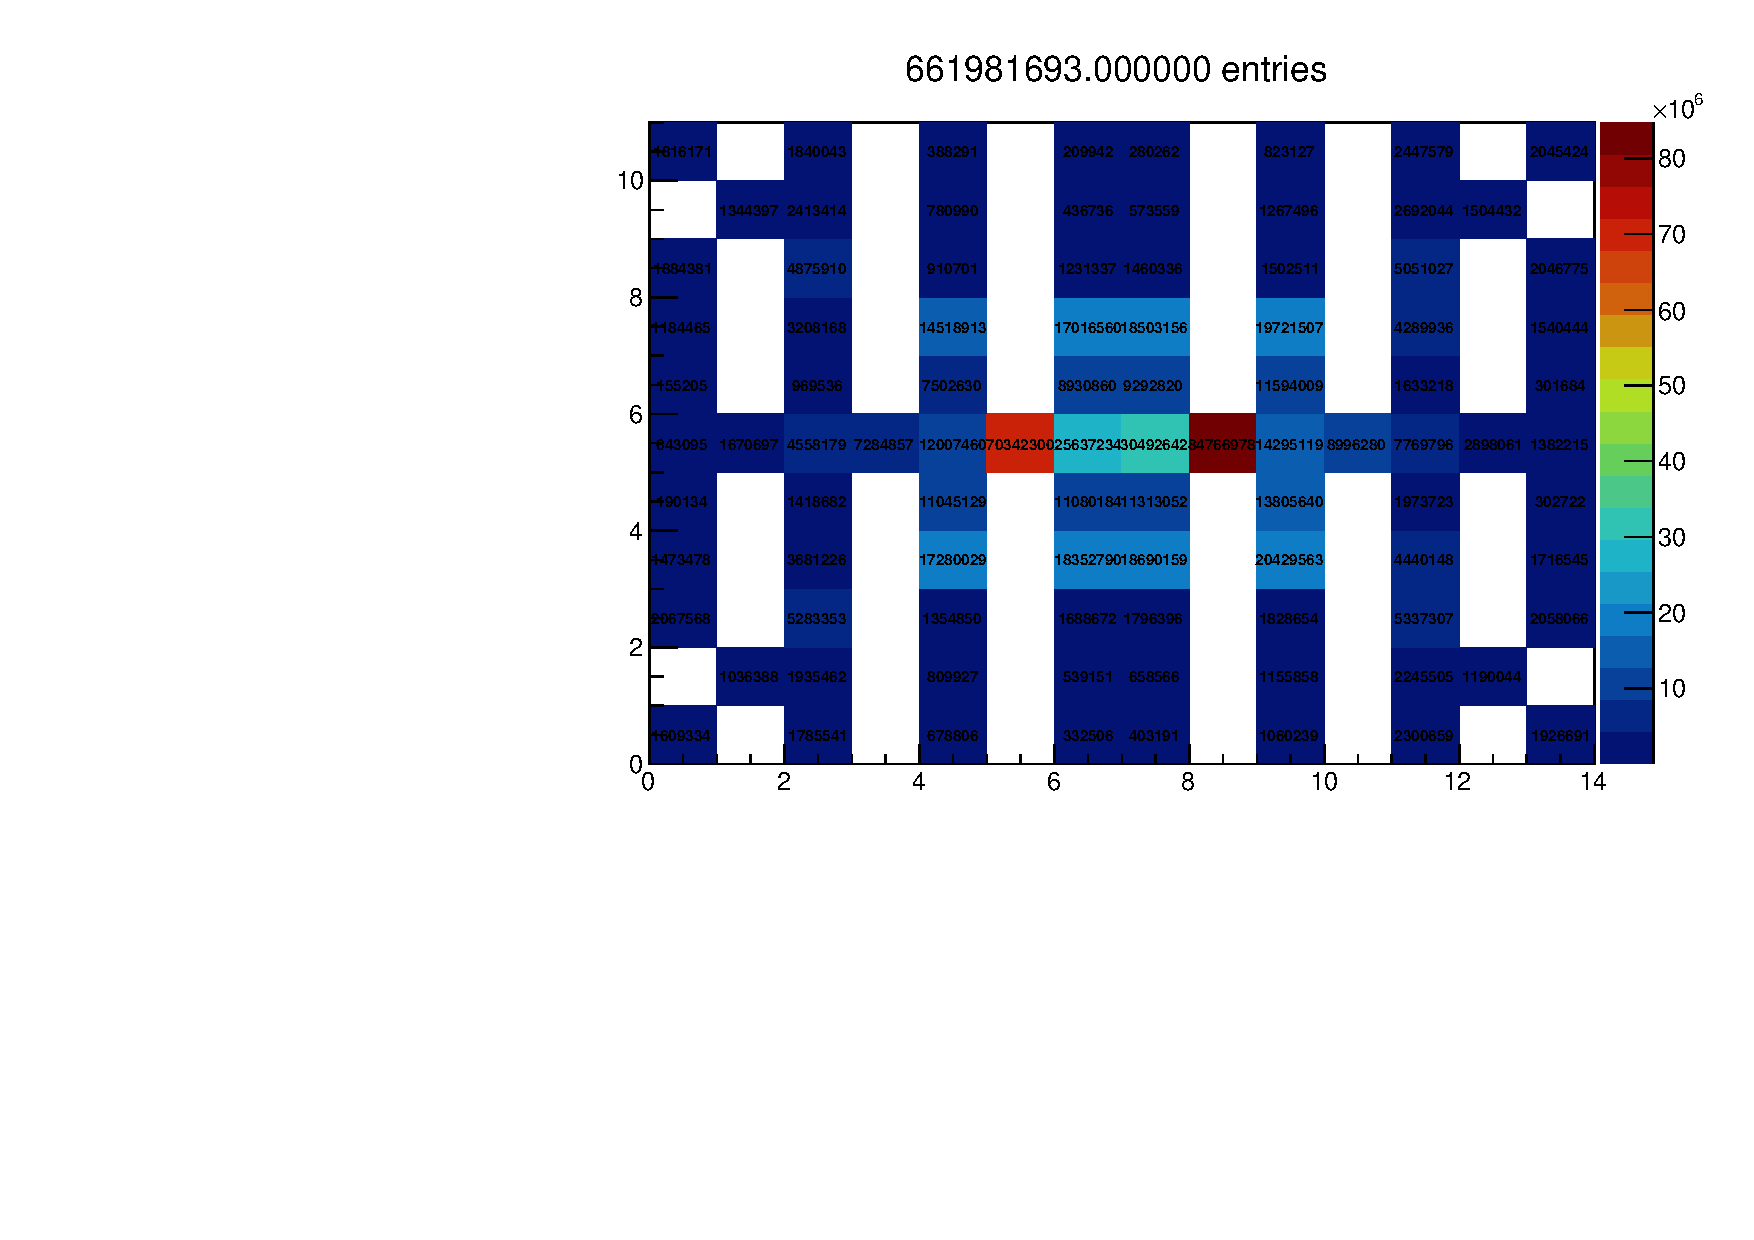
\includegraphics[width=0.48 \textwidth] {entries_rich2_19072015.pdf}}
		\subfigure{ 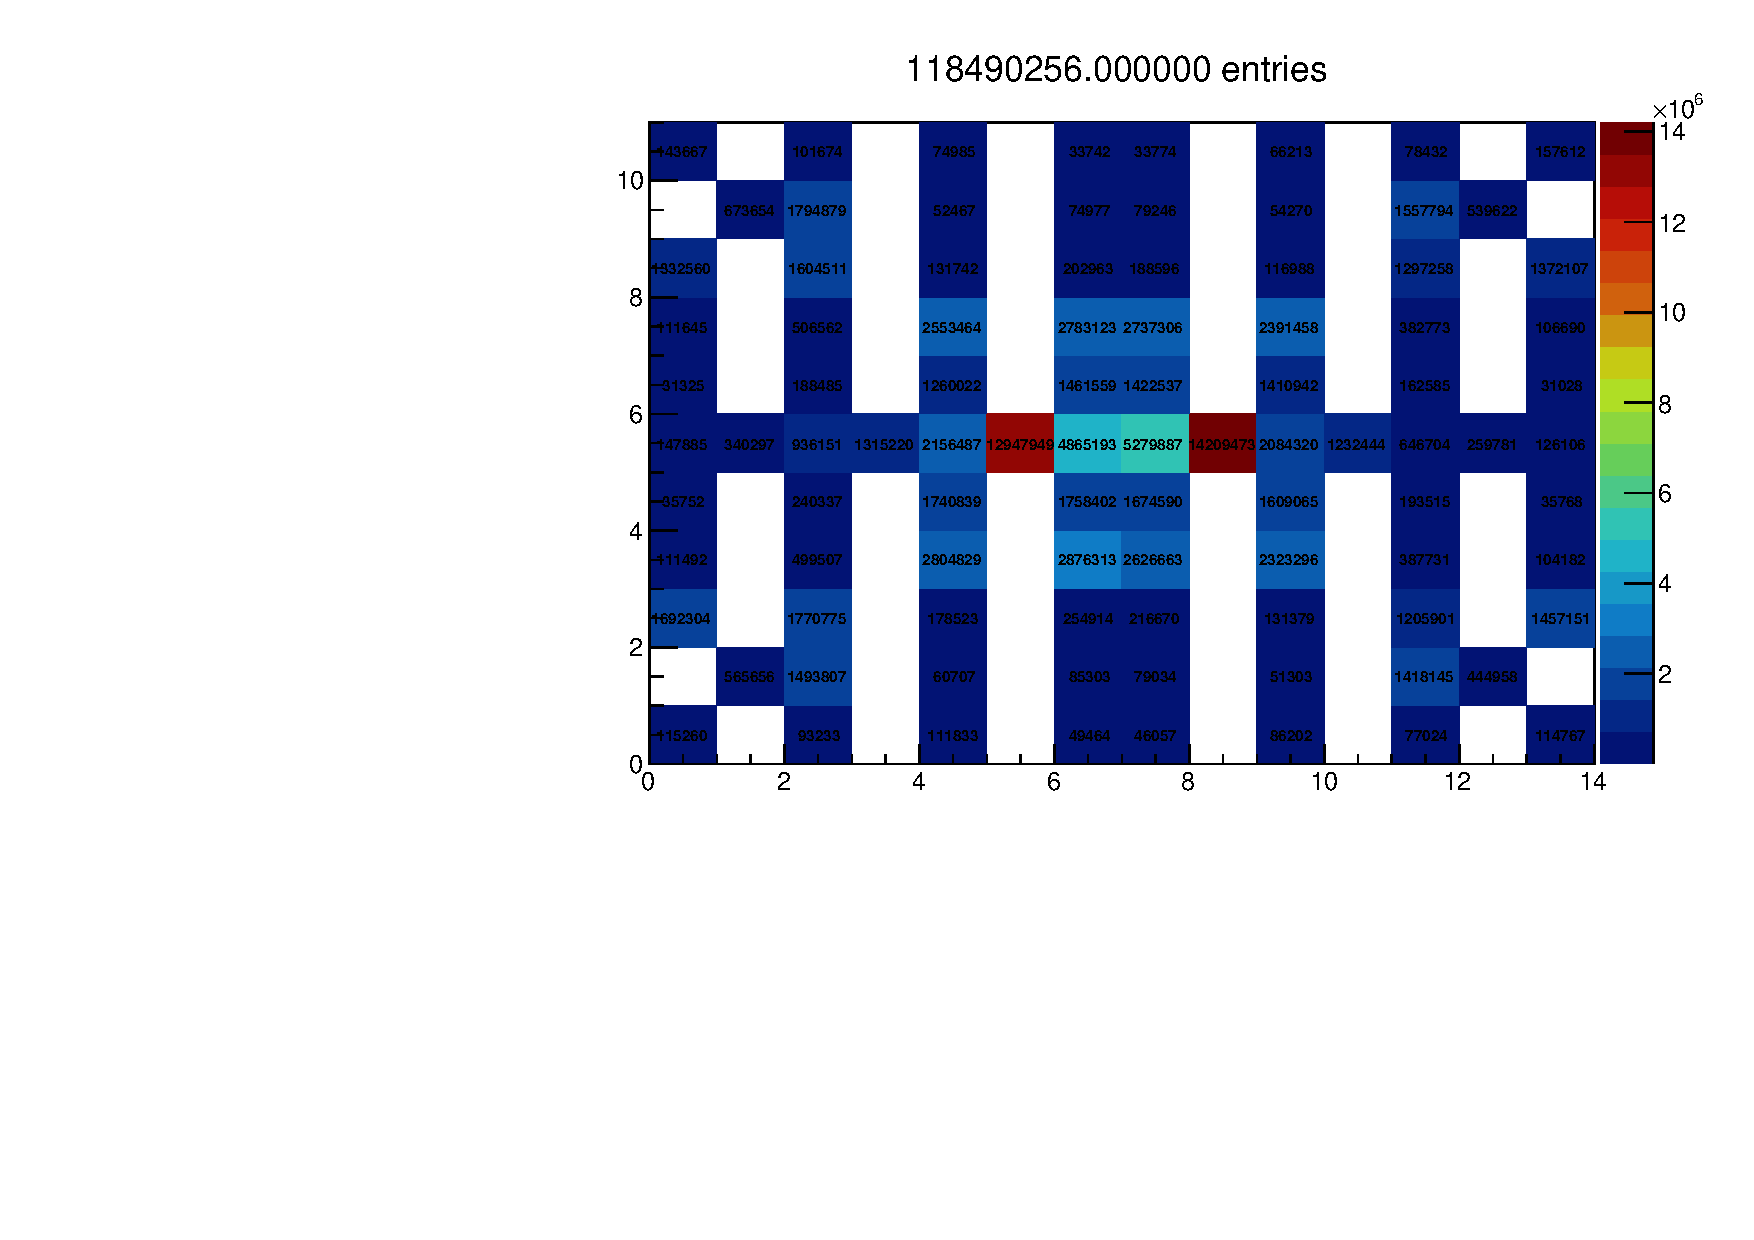
\includegraphics[width=0.48 \textwidth] {entries_rich2_09092015.pdf}}
		\vspace*{-0.5cm}
	\end{center}
	\caption{\textit{The number of unambiguous photon hits per mirror-pair for three different alignments. Top left:} \textbf{first alignment}\textit{; top right:} \textbf{second alignment}\textit{; bottom:} \textbf{third alignment}\textit{. The value in the title of each plot is the total number of unambiguous photons. } }
	\label{fig:rich2entries}
\end{figure}
Note that the RICH2 HLT line changed somewhere between the second and the third alignment.\\
\\

\clearpage

\section{Mag Down to Mag Up alignment}
The effect of the magnet polarity switch on the alignment has recently been tested. Chris applied the current alignment to the COLLISION15EM and COLLISION15 data. The distribution of the Cherenkov angle resolution for both RICH1 and RICH2 are shown in Figure \ref{fig:chris}. The magnet polarity flip happened at run 158517.\\
\begin{figure}[!h]
	\vspace*{-0.cm}
	\begin{center}
		\subfigure{ 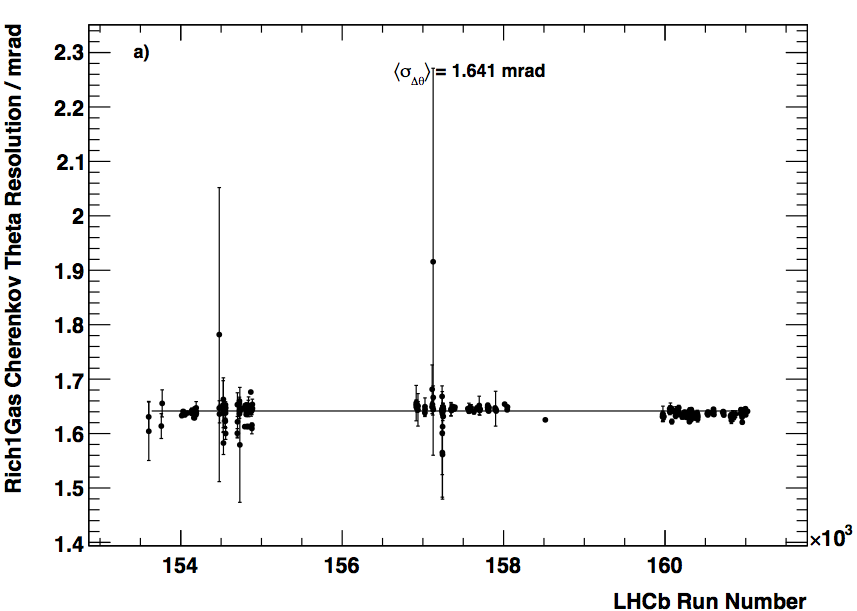
\includegraphics[width=0.48 \textwidth] {chrisrich1.png}}
		\subfigure{ 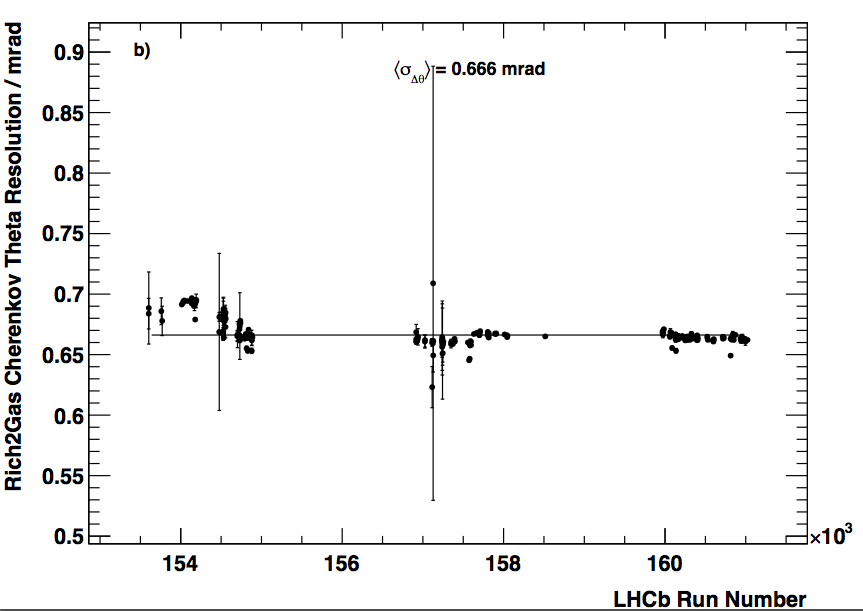
\includegraphics[width=0.48 \textwidth] {chrisrich2.png}}
		\vspace*{-0.5cm}
	\end{center}
	\caption{\textit{Cherenkov angle resolution by run for the currently used alignment in the database. Left: RICH1; Right: RICH2.} }
	\label{fig:chris}
\end{figure}

Starting from the current alignment made on the mag down data an alignment has been performed on the mag down data. Both RICH1 and RICH2 converged within 2 iterations (meaning mirrors were tilted only once).\\
The change in resolution with respect to the mag down alignment can be seen in Figure \ref{fig:rich1del} top right for RICH1 and in Figure \ref{fig:rich2del} bottom plot for RICH2. At the end of the current alignment the data sample it was \textit{trained} on (mag down data) obtained a resolution of $1.533 \pm 0.006\, mrad$. This alignment applied to the mag down data yielded a resolution of $1.529 \pm 0.007\, mrad$ which was improved to $1.527 \pm 0.004\, mrad$ after the alignment. For RICH2 the resolution of the current alignment on the data sample it was trained on (mag down data) is $0.5900 \pm 0.0004$. This alignment applied to the mag up sample yielded a resolution of $0.5909 \pm \, 0.0005$. At the end of the alignment to the mag up data the resolution was $0.5903 \pm 0.0005 \, mrad$. \\
This and Chris' plots give the impression that with the current procedure we can only align to the precision of $0.1 \, mrad$.\\

\subsection{Tilts in mirrors and changes of resolution}
During the alignment from mag down to mag up several mirror-pairs experienced tilts. \\
Comparing Table \ref{tab:rich1} with the bottom right plot of Figure \ref{fig:rich1del} you see that the biggest mirror tilts also show the biggest improvements in resolution. The big changes happen in the outer mirror though that have lower occupancy, thus the overall Cherenkov angle resolution doesn't change as much.\\

\begin{table}[!h]
	\begin{center}
		\begin{tabular}{c|c|c|c|c|c|c|c}
               -.2  &  .2  & -.2  &  .0  & \qquad   .1  &  .0  & -.1  &  .0 \\
               -.8  &  .0  & -.1  &  .0  & \qquad   -.2 &  -.1 &   .0 &  -.1 \\
               1.6  &  .0  &  .1  &  .2  &  \qquad 1.1  &  .0  &  .1  &  .0 \\
               -.3  &  .3  &  .2  &  .0 &   \qquad -.1  & -.2  &  .6  &  .0 \\
\end{tabular}
\end{center}
\caption{\textit{Truncated tilts for the secondary mirrors of RICH1 in mrad. Left columns: tilts in y; right columns: tilts in z. }}
\label{tab:rich1}
\end{table}

The same seems to be the case for RICH2. The mirrors that experience the biggest tilts are those on the outer edges which don't have a big impact on the overall Cherenkov angle resolution.\\

 \begin{table}[!h]
	\begin{center}
		\begin{tabular}{c|c|c|c|c|c|c|c|c|c|c|c|c|c|c|c}
    .0  &  .0  &  .0  &  .0 &   .0  &  .0  &  .0  &  .0 & \qquad      -.1  & -.1  &  .0  &  .0  &  .0  &  .0  &  .0  &  .0 \\
    .0  &  .0  &  .0  &  .0 &   .0  &  .0  &  .0  &  .0 & \qquad      -.2  & -.1  &  .0  &  .0  &  .0  &  .0  &  .0  & -.1\\
    .0  &  .0  &  .0  &  .0 &   .0  &  .0  &  .0  &  .0  & \qquad      .0  &  .0  &  .0  &  .0  &  .0  &  .0  &  .0  &  .0\\
    .0  &  .0  &  .0   & .0 &   .0  &  .0  &  .0  & -.1  & \qquad      .1  &  .0  &  .0  &  .0  &  .0  &  .0  &  .0  &  .0\\
    .0  &  .0  &  .0   & .0 &   .0  &  .0  &  .0  &  .0 & \qquad       .0  &  .0  &  .0  &  .0  &  .0  &  .0  &  .0  &  .0\\
    .0  &  .0  &  .0   & .0 &   .0  &  .0  &  .0  &  .0  & \qquad      .0  &  .0  &  .0  &  .0  &  .0  &  .0  &  .0  &  .1\\
    .0   & .0  &  .0   & .0 &   .0  &  .0  &  .0  &  .0  & \qquad      .0  &  .0  &  .0  &  .0  &  .0  &  .0  &  .0  &  .0 \\
\end{tabular}
\end{center}
\caption{\textit{Truncated tilts for the primary mirrors of RICH2 in mrad. Left columns: tilts in y; right columns: tilts in z. }}
\end{table}


\begin{table}[!h]
	\begin{center}
		\begin{tabular}{c|c|c|c|c|c|c|c|c|c|c|c|c|c|c|c}
	.0  &  .0  &  .0   & .0  &  .0  &  .0  &  .0  &  .0   & \qquad     .6  &  .4  & -.1  &  .0  &  .0  &  .0  &  .1  &  .3\\
    .0  &  .0  &  .0   & .0  &  .0  &  .0  &  .0  &  .0   & \qquad     .2  &  .1  &  .0  &  .0  &  .0  &  .0  &  .0  &  .3\\
    .0  &  .0  &  .0   & .0  &  .0  &  .0  &  .0  &  .0   & \qquad     .0  &  .0  &  .0  &  .0  &  .0  &  .0  &  .0  &  .0\\
    .0  &  .0  &  .0   & .0  &  .0  &  .0  &  .1  & -.1   & \qquad     .0  &  .0  &  .0  &  .0  &  .0  &  .0  &  .0  &  .0\\
    .1  &  .0  &  .0   & .0  &  .0   & .0  &  .0  & -.1   & \qquad    -.4  & -.2  &  .0  &  .0  &  .0  &  .1  & -.1  & -.1\\
    \end{tabular}
\end{center}
\caption{\textit{Truncated tilts for the secondary mirrors of RICH2 in mrad. Left columns: tilts in y; right columns: tilts in z. }}
\end{table}
